%% This is the ctufit-thesis example file. It is used to produce theses
%% for submission to Czech Technical University, Faculty of Information Technology.
%%
%% Get the newest version from
%% https://gitlab.fit.cvut.cz/theses-templates/FITthesis-LaTeX

% arara: xelatex
% arara: biber
% arara: xelatex
% arara: xelatex

%%%%%%%%%%%%%%%%%%%%%%%%%%%%%%%%%%%%%%%%%
% CLASS OPTIONS
% language: czech/english/slovak
% thesis type: bachelor/master/dissertation
% colour: bw for black&white OR no option for default colour scheme
% electronic (oneside) or printed (twoside), twoside is default
% paragraph - if passed, this optional argument sets paragraphs as the deepest level of headers, styles it, numbers it and adds it to Table of Content. Use with care! Normally, it is considered unwise to use it, since its too deep.
%%%%%%%%%%%%%%%%%%%%%%%%%%%%%%%%%%%%%%%%%
\documentclass[english,bachelor,bw,unicode,oneside]{ctufit-thesis}

%%%%%%%%%%%%%%%%%%%%%%%%%%%%%%%%%%
% FILL IN THIS INFORMATION
%%%%%%%%%%%%%%%%%%%%%%%%%%%%%%%%%%
\ctufitauthorsurnames{Laštovička}
\ctufittitle{NAC-colorings search: complexity and algorithms}
\ctufitauthorfull{Petr Laštovička}
\ctufitauthorgivennames{Petr}
\ctufitsupervisor{Dr.\,techn.\,Ing.\,Jan Legerský}
\ctufitdepartment{Faculty of Theoretical Informatics}
\ctufityear{2025}
\ctufitdeclarationplace{Prague}
\ctufitdeclarationdate{\today} % replace with the date of signature of the declaration
\ctufitabstractCZE{
    Jedna z otázek v strukturální teorii tuhosti (Rigidity Theory)
    je, zda realizace vrcholů grafu do roviny je flexibilní,
    tj.~zda umožňuje spojitou deformaci neměnící délku hran.
    %
    Flexibilní realizace souvislého grafu do roviny existuje právě tehdy, když
    graf má NAC-obarvení, hranové obarvení dvěma barvami takové,
    že pro každý cyklus jsou všechny hrany obarveny stejnou barvou nebo
    jsou každou barvou obarveny alespoň dvě hrany.
    %
    Je NP-úplné rozhodnout, zda graf má NAC-obarvení, v práci ukazujeme,
    že problém je NP-úplný i pro grafy s maximálním stupněm pět.
    %
    Představujeme značně rychlejší algoritmus na hledání NAC-obarvení společně s různými heuristikami.
    Srovnáváme ho s předchozími algoritmy a porovnáváme i heuristiky mezi sebou.
    %
    Následně představujeme FPT algoritmus na počítání NAC-obarvení
    parametrizovaný stromovou šířkou.
    %
    % Navíc popisujeme vztahy s stable řezy grafu a implementujeme algoritmus
    % pro jejich hledání v flexible grafech.
}
% Also update README.md if any changes are made.
\ctufitabstractENG{
    One of the questions in Rigidity Theory is whether a realization of the
    vertices of a graph in the plane is flexible, namely, if it allows a continuous
    deformation preserving the edge lengths.
    %
    A flexible realization of a connected graph in the plane exists if and only if
    the graph has a NAC-coloring, which is surjective edge coloring by
    two colors such that for each cycle either all the edges have the same color or
    there are at least two edges of each color.
    %
    It is \mbox{NP-complete} to determine is a graph has a NAC-coloring,
    we show that the problem is
    also NP-complete for graphs with maximal degree five.
    %
    We present a significantly faster algorithm for NAC-coloring search,
    and we discuss related heuristics.
    The performance is compared with previous algorithms and among the heuristics.
    %
    After, we present another FPT algorithm for NAC-coloring counting
    parametrized by tree width.
    %
    % We also discuss relation to stable cuts and algorithm for finding
    % a stable cut is implemented as part of the thesis.
}

\ctufitkeywordsCZE{
    strukturální teorie tuhosti,
    generická flexibilita,
    NAC-barvení,
    stable-cut,
    parametrizovaná komplexita,
    NP-úplnost
}
\ctufitkeywordsENG{
    rigidity theory,
    generic flexibility,
    NAC-coloring,
    stable-cut,
    pa\-rametrized complexity,
    NP-completeness
}
%%%%%%%%%%%%%%%%%%%%%%%%%%%%%%%%%%
% END FILL IN
%%%%%%%%%%%%%%%%%%%%%%%%%%%%%%%%%%

%%%%%%%%%%%%%%%%%%%%%%%%%%%%%%%%%%
% CUSTOMIZATION of this template
% Skip this part or alter it if you know what you are doing.
%%%%%%%%%%%%%%%%%%%%%%%%%%%%%%%%%%

\RequirePackage{iftex}[2020/03/06]
\iftutex{}% XeLaTeX and LuaLaTeX
    \RequirePackage{ellipsis}[2020/05/22] %ellipsis workaround for XeLaTeX
\else
    \errmessage{Only compilation with XeLaTeX or LuaLaTeX is allowed}
    \stop
\fi

% hyperlinks
\hypersetup{
    pdfpagelayout=TwoPageRight,
    colorlinks=false,
    allcolors=decoration,
    pdfborder={0 0 0.1}
}

% uncomment the following to hide all hyperlinks
%\hypersetup{hidelinks}

% uncomment the following to change the color of all hyperlinks to CTU blue
\hypersetup{allbordercolors=decoration}

\RequirePackage{pdfpages}[2020/01/28]

%%%%%%%%%%%%%%%%%%%%%%%%%%%%%%%%%%
% CUSTOMIZATION of this template END
%%%%%%%%%%%%%%%%%%%%%%%%%%%%%%%%%%


%%%%%%%%%%%%%%%%%%%%%%
% CONTENTS SETTINGS
%%%%%%%%%%%%%%%%%%%%%%
\usepackage{dirtree}
\usepackage{lipsum,tikz}
\usepackage{xurl}
\usepackage{listings} % typesetting of sources
%\usepackage{minted}
\usepackage{csquotes}
% Handles czech line breaks
% \usepackage{xevlna}
\usepackage{pdflscape}
\usepackage{hyperref}
\usepackage[nameinlink]{cleveref}

\usepackage{todonotes}

\usepackage[style=iso-numeric]{biblatex}
\addbibresource{./text/bib-database.bib}
%%%%%%%%%%%%%%%%%%%%%%
% CONTENTS SETTINGS END
%%%%%%%%%%%%%%%%%%%%%%

%%%%%%%%%%%%%%%%%
% CUSTOM COMMANDS
%%%%%%%%%%%%%%%%%

% Text mode macros
\newcommand{\WLOG}{WLOG}
\newcommand{\G}{\(G\)}
\newcommand{\Gprime}{\(G^\prime\)}
\newcommand{\Ered}{E_\text{red}}
\newcommand{\Eblue}{E_\text{blue}}
%% FPT
\newcommand{\MSO}{\(\text{MSO}_2\)}
\newcommand{\Xt}{\(X_t\)}
\newcommand{\LeafNode}{\textsc{Leaf Node}}
\newcommand{\RootNode}{\textsc{Root Node}}
\newcommand{\IntroduceVertexNode}{\textsc{Introduce Vertex Node}}
\newcommand{\ForgetVertexNode}{\textsc{Forget Vertex Node}}
\newcommand{\IntroduceEdgeNode}{\textsc{Introduce Edge Node}}
\newcommand{\JoinNode}{\textsc{Join Node}}
\newcommand{\IntroduceVertexWithEdgesNode}{\textsc{Introduce Vertex With Edges Node}}

% Math mode macros
\newcommand{\red}{\text{red}}
\newcommand{\blue}{\text{blue}}
\newcommand{\NAC}{\text{NAC}}
\newcommand{\NACno}{\text{NAC}_\#}
\newcommand{\N}{\mathbb{N}}
\newcommand{\R}{\mathbb{R}}
\newcommand{\inc}{\text{inc}}
\newcommand{\pluseq}{\mathrel{+}=}
%% Stable cuts
\newcommand{\GSC}{\mathcal{G}_{sc}}


%%%%%%%%%%%%%%%
\colorlet{ecol}{black!50!white}
\definecolor{colR}{rgb}{.932,.172,.172} %x11 Firebrick2
\definecolor{colB}{rgb}{.255,.41,.884} %svgnames RoyalBlue
\definecolor{colOrange}{RGB}{255,191,0} %Amber
%% Tikz styles
\tikzstyle{vertex}=[circle, draw, fill=black, inner sep=0pt, minimum size=4pt]
\tikzstyle{vertexSig}=[circle, draw, fill=colOrange, inner sep=0pt, minimum size=4pt]
\tikzstyle{edge}=[line width=1.5pt,ecol]
% dotted, densely dotted, loosely dotted, dashed
\tikzstyle{dots}=[dotted dash=1.5pt]
\tikzstyle{redge}=[edge,colR]
\tikzstyle{bedge}=[edge,colB]
\tikzstyle{yedge}=[edge,colOrange]

%%%%%%%%%%%%%%%%%
% CUSTOM COMMANDS END
%%%%%%%%%%%%%%%%%


\begin{document}
\frontmatter\frontmatterinit{} % do not remove these two commands

\thispagestyle{empty}\maketitle\thispagestyle{empty}\cleardoublepage{} % do not remove these four commands

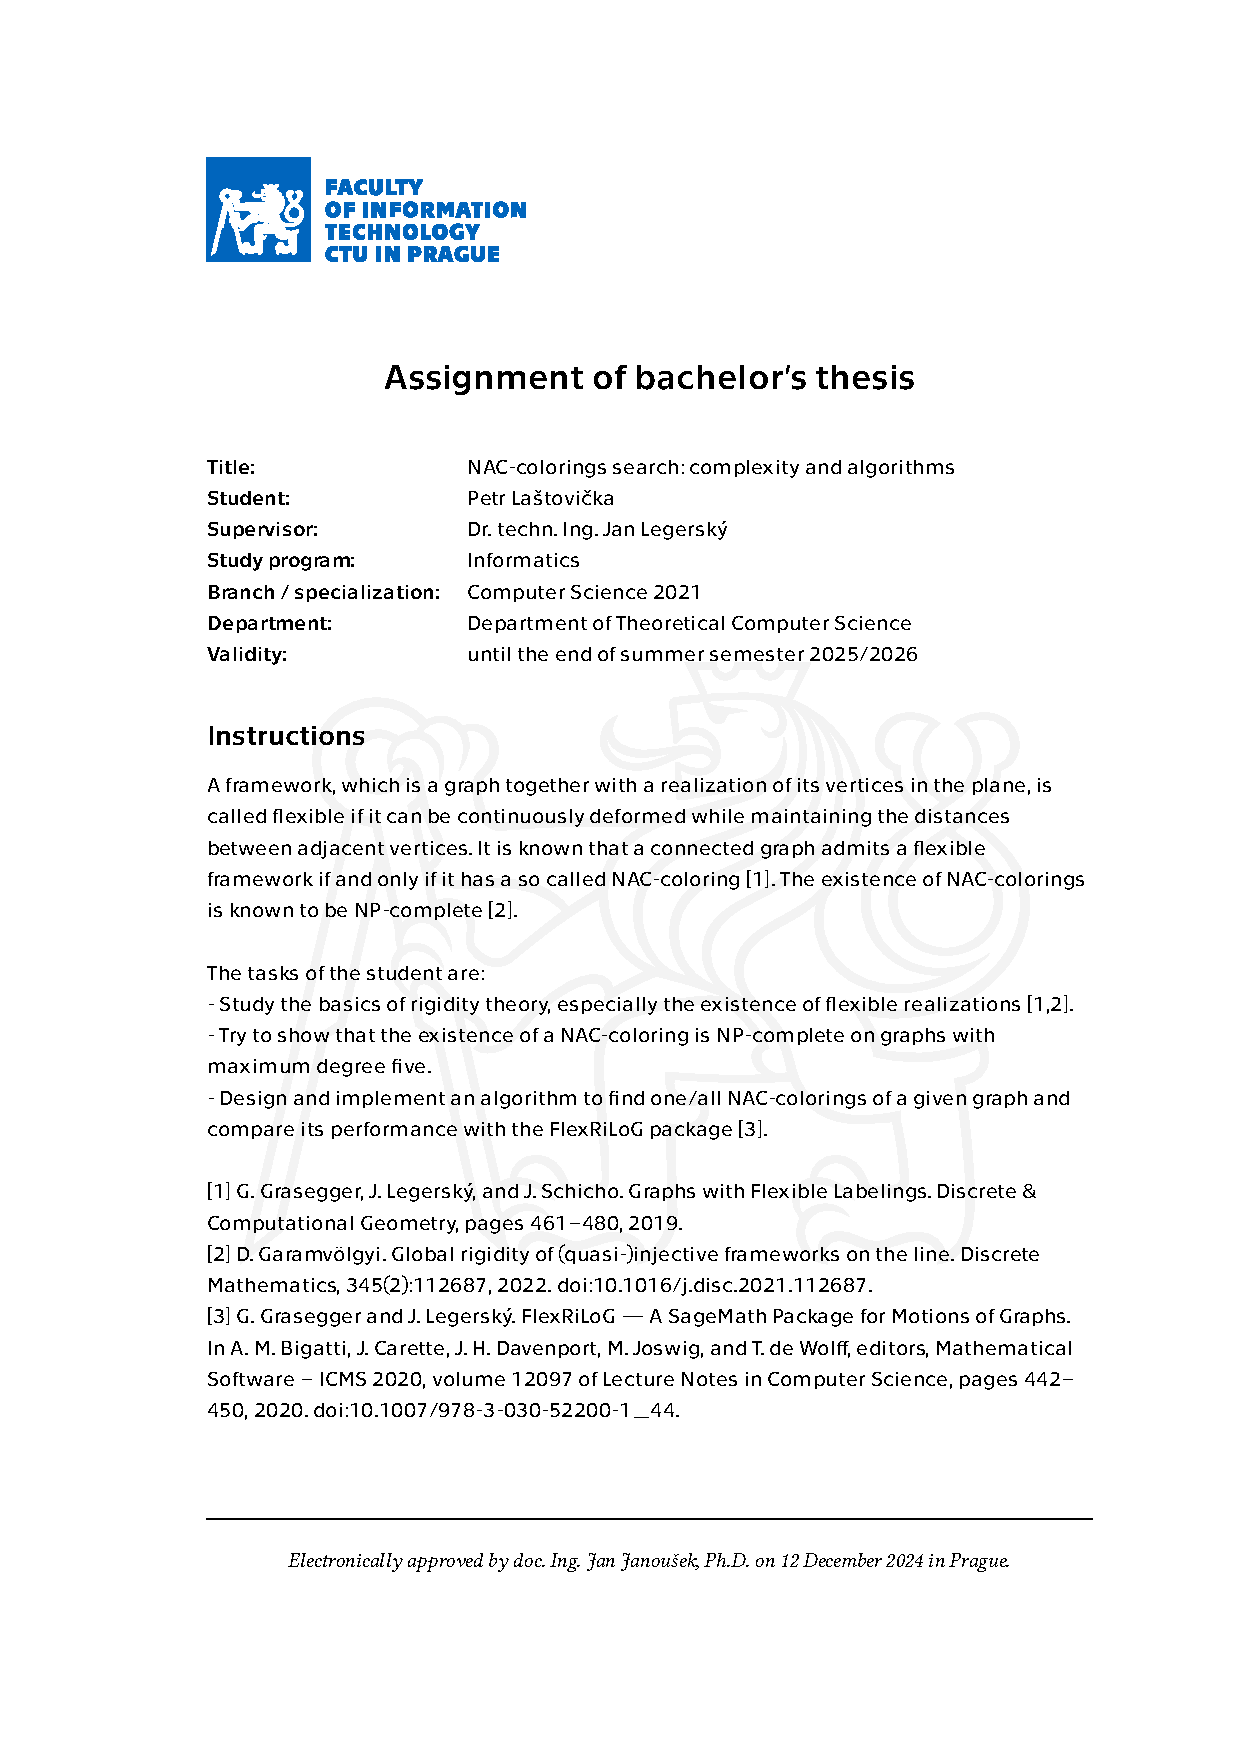
\includepdf[pages={1-}]{./assignment.pdf} % thesis assignment generated from ProjectsFIT

\imprintpage{} % do not remove this command
\stopTOCentries % TODO This should not be removed!

%%%%%%%%%%%%%%%%%%%%%%
% list of other contents END
%%%%%%%%%%%%%%%%%%%%%%

%%%%%%%%%%%%%%%%%%%
% ACKNOWLEDGMENT
% This is a place to thank people for helping you. It is common to thank your supervisor.
%%%%%%%%%%%%%%%%%%%
\begin{acknowledgmentpage}
	Chtěl bych poděkovat především sit amet, consectetuer adipiscing elit. Curabitur sagittis hendrerit ante. Class aptent taciti sociosqu ad litora torquent per conubia nostra, per inceptos hymenaeos. Cras pede libero, dapibus nec, pretium sit amet, tempor quis. Sed vel lectus. Donec odio tempus molestie, porttitor ut, iaculis quis, sem. Suspendisse sagittis ultrices augue.

	Vedoucí
	Michal Opler za nápad FTP
	Knop za materiály
	Rodina
	Přátelé
	Učitelům KTI a KAM
\end{acknowledgmentpage}
%%%%%%%%%%%%%%%%%%%
% ACKNOWLEDGMENT END
%%%%%%%%%%%%%%%%%%%


%%%%%%%%%%%%%%%%%%%
% DECLARATION
% FILL IN / MODIFY
%%%%%%%%%%%%%%%%%%%
% INSTRUCTIONS
% https://courses.fit.cvut.cz/SFE/download/index.html#_documents () (prohlášení do ZP)
\begin{declarationpage}
	I hereby declare that the presented thesis is my own work and that I have cited all sources of
	information in accordance with the Guideline for adhering to ethical principles when elaborating an
	academic final thesis.

	I acknowledge that my thesis is subject to the rights and obligations stipulated by the Act No.
	121/2000 Coll., the Copyright Act, as amended. In accordance with Section 2373(2) of Act No.
	89/2012 Coll., the Civil Code, as amended, I hereby grant a non-exclusive authorization (license) to
	utilize this thesis, including all computer programs that are part of it or attached to it and all
	documentation thereof (hereinafter collectively referred to as the ``Work''), to any and all persons
	who wish to use the Work. Such persons are entitled to use the Work in any manner that does not
	diminish the value of the Work and for any purpose (including use for profit). This authorization is
	unlimited in time, territory and quantity
\end{declarationpage}
%%%%%%%%%%%%%%%%%%%
% DECLARATION END
%%%%%%%%%%%%%%%%%%%

\printabstractpage{} % do not remove this command

%%%%%%%%%%%%%%%%%%%
% SUMMARY
% FILL IN / MODIFY
% OR REMOVE ENTIRELY (upon agreement with your supervisor)
% (appropriate to remove in most theses)
%%%%%%%%%%%%%%%%%%%
% \begin{summarypage}
% \section*{Summary section}
% 
% \lipsum[1][1-8]
% 
% \section*{Summary section}
% 
% \lipsum[2][1-6]
% 
% \section*{Summary section}
% 
% \lipsum[3]
% 
% \section*{Summary section}
% 
% \lipsum[2]
% 
% \section*{Summary section}
% 
% \lipsum[1][1-8] Lorem lorem lorem.
% \end{summarypage}
%%%%%%%%%%%%%%%%%%%
% SUMMARY END
%%%%%%%%%%%%%%%%%%%

\tableofcontents % do not remove this command
%%%%%%%%%%%%%%%%%%%%%%
% list of other contents: figures, tables, code listings, algorithms, etc.
% add/remove commands accordingly
%%%%%%%%%%%%%%%%%%%%%%
\listoffigures % list of figures
\begingroup
\let\clearpage\relax
\listoftables % list of tables
\thectufitlistingscommand{}
\endgroup

%%%%%%%%%%%%%%%%%%%
% ABBREVIATIONS
% FILL IN / MODIFY
% OR REMOVE ENTIRELY
% List the abbreviations in lexicography order.
%%%%%%%%%%%%%%%%%%%
\chapter{\thectufitabbreviationlabel}

\begin{tabular}{rl}
	FPT    & Fixed-parameter tractable            \\
	\MSO{} & Monadic second-order logic on graphs \\
	NAC    & No almost cycles                     \\
\end{tabular}
%%%%%%%%%%%%%%%%%%%
% ABBREVIATIONS END
%%%%%%%%%%%%%%%%%%%
\resumeTOCentries{}
\mainmatter\mainmatterinit{} % do not remove these two commands
%%%%%%%%%%%%%%%%%%%
% THE THESIS
% MODIFY ANYTHING BELOW THIS LINE
%%%%%%%%%%%%%%%%%%%


\chapter{Introduction}
% uncomment the following line to create an unnumbered chapter
%\chapter*{Introduction}\addcontentsline{toc}{chapter}{Introduction}\markboth{Introduction}{Introduction}
\setcounter{page}{1}

% Pohádka
% Nepřehánět to s definicemi a citacemi -> spíše teoretická část
% Proč to dělám, význam, návaznost (PyRigi)
% Jak jsem si to vybral
% prodat drony
% Cíle
% - část úvodu, nebo vlastní kapitola
% Obsah jen stručně

The core concept of Rigidity Theory is a \emph{framework} of a simple graph \(G\).
It is a realization of \(G\) into a \(d\)-dimensional plane \(p: V(G) \to \R^d\).
A framework is \emph{\( d \)-flexible} if there exists a transformation
that continuously translates some subset of vertices in such a way that
distances between neighboring vertices are preserved during the transformation.
Otherwise, the framework is called \emph{\( d \)-rigid}.

For \( d = 1 \) all the vertices are on a line
and any vertex deviation necessarily changes distances (if the graph is connected).
%
For \( d \ge 3 \) we can map all the vertices except one onto a line and
rotate the vertex around the line.
%
The interesting case is when \( d = 2 \) --- a mapping into a plane.
It is known that a graph has most of the realizations
either \( 2 \)-flexible, or \( 2 \)-rigid,
still there may be some realizations of the other type~\cite{generically_rigid_graphs}
--- we talk about paradoxical flexibility.
A graph is \emph{(generically) rigid} if most of the realizations are \( 2 \)-rigid
and \emph{(generically) flexible} if most of the realizations are \( 2 \)-flexible.

An example application of the Rigidity Theory is a squadron of drones
where the drones can measure distance to their close neighbors.
Can we determine the locations of all the drones
down to translation and rotation of the whole squadron
just from such information?

For similar problems in the plane,
one would think that if the graph formed is rigid, the answer is yes, and
for flexible graphs the answer is no.
But as stated above, paradoxically even a rigid graph can have a flexible realization,
and it may just happen that the drones form such a \( 2 \)-flexible framework.

In efforts to find such paradoxical realizations,
a new edge coloring was defined~\cite{legersky_original}.
A \emph{NAC-coloring} is an edge coloring of a graph by \( \red \) and \( \blue \)
such that both the colors are used and there is no almost cycle formed.
An \emph{almost cycle} is a cycle in the colored graph such that exactly one
edge of the cycle is colored \( \red \) or exactly one edge is colored \( \blue \).
Such coloring exists if and only if the graph has a flexible realization.
This provides a simple but strong tool to decide whenever a graph has
a flexible realization even if it is rigid.
As shown later in the thesis, one can check in polynomial time if a coloring
given is a NAC-coloring.
Unfortunately, it is NP-complete to decide if a graph has any NAC-coloring.

\begin{figure}[ht]
	\centering
	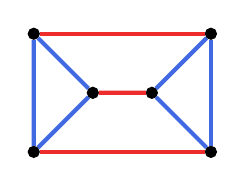
\begin{tikzpicture}[rotate=90,scale=1.5]
		\node[vertex] (a) at (0,0) {};
		\node[vertex] (b) at (1,0) {};
		\node[vertex] (c) at (0.5,0.5) {};
		\node[vertex] (d) at (0,1.5) {};
		\node[vertex] (e) at (1,1.5) {};
		\node[vertex] (f) at (0.5,1) {};
		\draw[bedge] (a)edge(b) (b)edge(c) (c)edge(a) (d)edge(e) (e)edge(f) (f)edge(d) ;
		\draw[redge] (a)edge(d) (b)edge(e) (c)edge(f);
	\end{tikzpicture}
	\qquad
	\qquad
	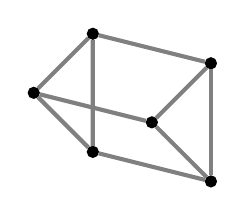
\begin{tikzpicture}[rotate=90,scale=1.5]
		\node[vertex] (a) at (0.00,0) {};
		\node[vertex] (b) at (1.00,0) {};
		\node[vertex] (c) at (0.50,0.5) {};
		\node[vertex] (d) at (0.25,1) {};
		\node[vertex] (e) at (1.25,1) {};
		\node[vertex] (f) at (0.75,1.5) {};
		\draw[edge] (a)edge(b) (b)edge(c) (c)edge(a) (d)edge(e) (e)edge(f) (f)edge(d) ;
		\draw[edge] (a)edge(d) (b)edge(e) (c)edge(f);
	\end{tikzpicture}
	\caption{The $3$-prism is generically $2$-rigid, but has a flexible realization (right).
		It has a unique NAC-coloring modulo swapping colors (left).}%
	\label{fig:3prism}
\end{figure}

A nice example for NAC-coloring showcase is the prism graph~\Cref{fig:3prism},
a graph formed from two triangles with three interconnecting edges.
Such graph is rigid, still it has a NAC-coloring and flexible realizations.
The flexible realizations are all the realization where
the triangles are identical except for translation.
You can check yourself that there are
no other NAC-colorings except the symmetric one.

The goals of this thesis are to provide an algorithm
that can find all the NAC-colorings of a graph.
Multiple heuristics will be used to significantly
reduce the runtime of the algorithm.
We also provide parametrized approach where complexity can be reduced for graphs
with low internal structural complexity (tree width).
We also show that the problem of deciding if a graph has a NAC-coloring
is NP-complete even on graphs with maximal degree five.
Later also show relation to stable cuts~\cite{stable_cuts_2v_4}.
Code implemented in this thesis will enrich the existing PyRigi~\cite{pyrigi}
library for Rigidity Theory.
Currently, there are no such algorithms implemented in PyRigi itself,
the only known implementation is rather naive in FlexRiLoG~\cite{flexrilog}.
We compare our implementation performance with FlexRiLoG and also compare
individual heuristics among each other.
Multiple relevant graph classes will be considered.

We summarize and extend our previous research done
on the topic in~\cite{my_paper}.



\chapter{Preliminaries}

\begin{chapterabstract}

	In this chapter we define terminology from Rigidity theory including NAC-coloring.
	We also introduce its relation to Rigidity theory and
	some simple statements considering
	structure of graphs and NAC-coloring existence.

\end{chapterabstract}

\section{Rigidity theory}

Rigidity theory, often also called Structural rigidity,
is a branch of combinatorial theory,
which studies properties of objects formed from flexible joins and rigid bars.
These objects can be represented as graphs with
a mapping into \( d \)-dimensional space.
Rigidity theory studies if such objects are rigid, or flexible.

For the rest of the thesis,
we consider only simple undirected graphs.
Often, only connected graphs are considered as disconnected graphs
represent uninteresting trivial cases.
By \( V(G) \) we denote vertices of a graph \( G \) and
by \( E(G) \) we denote edges of a graph \( G \).
The following definitions are inspired by~\cite{np_complete,my_paper}.

%
\begin{definition}[\( d \)-realization]
	\emph{A \( d \)-realization} of a graph \( G \) is a mapping \( p: V(G) \to \R^d \).
\end{definition}
%
\begin{definition}[Framework]
	\emph{A framework} is a pair of a graph \( G \) and its realization.
\end{definition}
%
\begin{definition}[Nontrivial flex]
	For a framework \( (G, p) \), \emph{a nontrivial flex} of
	\( p_0 = p \) such that for all \( 0 < t \le 1 \) we have \( p_t \) such that
	\( \|p_t(u) - p_t(v)\| = \|p(u) - p(v)\|\) for every \( \{u, v\} \in E(G) \),
	but \( \|p_t(u) - p_t(v)\| \ne \|p(u) - p(v)\| \) for some \( u, v \in V (G) \).
\end{definition}
%
\begin{definition}[\( d \)-flexible, \( d \)-rigid]
	A framework is \( d \)-flexible, if it has a nontrivial flex.
	Otherwise, it is \( d \)-rigid.
\end{definition}
%
To summarize all the previous definitions,
a framework is flexible if it can be deformed while preserving lengths of
edges of the graph.

From now on we consider only \emph{quasi-injective} realizations ---
two neighboring vertices cannot be mapped to the same position.
This is guarantied when distances of neighboring vertices are positive.
Note that two non-neighboring vertices can be mapped to the same position.
Similar results can be shown for frameworks with \emph{injective} realizations
\todo[inline]{Footnote
	% \footnote{
	For example, it is also NP-complete to
	recognize graphs that have a generically rigid injective realization in \( \R^1 \).
	% }.
}
In this thesis they are of no interest for us.

It is NP-hard to decide whether a given \( d \)-dimensional framework is
\( d \)-rigid for \( d \ge 2 \)~\cite{d_rigidity_hardness}.
We can simplify the problem if we talk about \emph{generic}
behavior.
%
\begin{definition}[Flexible \& Rigid graphs~\cite{generically_rigid_graphs}]
	A graph is \( (generically) flexible \) if almost all of
	its \( 2 \)-realizations are \( 2 \)-flexible.
	A graph is \( (generically) rigid \) if almost all of
	its \( 2 \)-realizations are \( 2 \)-rigid.
\end{definition}
%

From now on we focus only on the \( 2 \)-dimensional case,
in which there is a combinatorial characterization of rigid graphs.

There is a significant graph class studied in Rigidity theory
called minimally rigid graphs or Laman graphs.
This class was described by Pollaczek-Geiringer~\cite{polzacek_1927}
and Laman~\cite{laman_1970} independently.
%
\begin{definition}
	Graph is \emph{minimally generically \( d \)-rigid} if it is \( d \)-rigid
	and \( G - e \)\footnote{
		\( G - e \) denotes a graph formed from \( G \) by removing an edge \( e \).
		Formally, \( G - e = (V(G), E(G) \setminus \{e\}) \).
	}
	is \(d\)-flexible for each \( e \in E(G) \).
\end{definition}
%
% \begin{theorem}[Pollaczek-Geiringer/Laman]
% 	There is a polynomial time algorithm for deciding if a graph is minimally
% \end{theorem}

It is already known for some classes of graphs that they are flexible.
Namely, graphs where \( |E(G)| \le 2|V(G)| - 4 \)
are flexible~\cite{stable_cuts_2v_4}.

A polynomial algorithm for testing \( 2 \)-rigidity was obtained
for minimally rigid graphs in~\cite{polynomial-min-rigid}.
We focus on these graphs in benchmarks.

\section{NAC-coloring}

It is algorithmically hard to find flexible realizations of a graph
just by trying realizations and checking if they are flexible
as the plane is continuous.
In~\cite{legersky_original} a new edge coloring is proposed
that corresponds with existence of a flexible realization.

\begin{definition}[NAC-coloring~\cite{legersky_original}]
	Let \( G \) be a graph and \( \delta: E(G) \to \{ \red, \blue \} \)
	be a coloring of edges:
	%
	\begin{itemize}
		\item A cycle in \( G \) is a \( \red \) cycle, if all its edges are \( \red \).
		\item A cycle in \( G \) is an \emph{almost \( \red \) cycle},
		      if exactly one of its edges is \( \blue \).
		      \emph{Almost \( \blue \) cycle} is defined analogously.
	\end{itemize}
	%
	By \emph{an almost cycle} we denote both almost \( \red \) and almost \( \blue \) cycles.
	A coloring \( \delta \) is called a NAC-coloring, if it is surjective
	and there are no almost cycles.
\end{definition}
%

It was shown in~\cite{np_complete}, that it is NP-complete to decide if a graph has a NAC-coloring.
We elaborate further on this in later chapters.
Thanks to the following \Cref{lemma:is_nac_coloring},
the check if a coloring is a NAC-coloring can be done in polynomial time.
Let \( E_\red\), resp. \( E_\blue \), be edges colored by \( \red \), resp.~\( \blue \),
in an edge coloring \( \delta \).
%
\begin{lemma}[\cite{legersky_original}]%
	\label[lemma]{lemma:is_nac_coloring}
	Let \( G \) be a graph. If \( \delta: E(G) \to \{ \red, \blue \} \) is a coloring of edges,
	then there are no almost cycles in \( G \) if and only if the connected components
	of \( G[E_\red] \) and \( G[E_\blue] \)%
	\footnote{
		For \(X \subseteq V(G)\), by \(G[X]\) we denote
		the induced subgraph of \( G \) on vertices \( X \),
		\( G[X] = (X, \{ \{u, v\} \mid u, v \in X\}) \).
		%
		For \(Y \subseteq E(G)\), by \(G[Y]\) we denote
		the induced subgraph of \( G \) on edges \( Y \),
		\( G[Y] = (\{ v \mid \exists u \in V(G) : \{u, v\} \in Y\}, Y) \).
	}
	are induced subgraphs of \( G \).
\end{lemma}
%
The idea is quite simple --- if there is w.l.o.g.\ \( \blue \) edge \( \{u, v\} \)
and \( \{u, v\} \) share the same connected component in \( G[E_\red] \),
an almost cycle is formed from a \( u \)-\( v \)-path in \( G[E_\red] \)
and the edge \( \{u, v\} \).

Now we present relation of NAC-colorings and flexible frameworks.
%
\begin{theorem}[\cite{legersky_original}]
	A connected graph \( G \) with at least one edge has a flexible
	quasi-injective \( 2 \)-dimensional realization if and only if it has a NAC-coloring.
\end{theorem}
%
The theorem has a constructive proof from which a flexible realization
can be found for a given NAC-coloring.
The proof itself is nontrivial, and we do not show it here.
For us the most interesting questions are whether a graph has a NAC-coloring
and how many NAC-coloring does a graph have.
For an example have a look at~\Cref{fig:3prism}
from Introduction.

Note that for each NAC-coloring \( \delta \) on graph \( G \)
there exists a NAC-coloring \( \delta^\prime \) on \( G \)
where \( \red \) and \( \blue \) colors are swapped.
%
\begin{definition}
	By \( \nac{G} \) we denote the set of all the NAC-coloring of graph \( G \).
	By \( \nnac{G} \) we denote the number of NAC-colorings of \( G \)
	up to swapping the colors.
	That is \( \nnac{G} = | \nac{G} | / 2 \)
\end{definition}
%

\subsection{NAC-coloring constraints}

In algorithms related to NAC-coloring search it is beneficial
to reduce the search space.
It can be often seen from the graph's structure
that if colors differ for some set of edges,
the resulting coloring cannot be a NAC-coloring.

All the edges of a 3-cycle subgraph \( C_3 \) must map to the same color.
Otherwise, two edges of \( C_3 \) are w.l.o.g.\ \( \red \) and one is \( \blue \).
Therefore, \( C_3 \) forms an almost cycle.
This idea can be expanded further to neighboring triangles.
%
\begin{definition}[\( \triangle \)-connected component~\cite{legersky_original}]
	\label[definition]{def:triangle_connected_component}
	Let \( G \) be a graph and \( \sim^\prime_\triangle \) be
	a relation on \( E(G) \times E(G) \) such that \( e_1 \sim^\prime_\triangle e_2 \)
	iff there exists a 3-cycle subgraph \( C_3 \) of \( G \)
	such that \( e_1, e_2 \in E(C_3) \).
	Let \( \sim_\triangle \) be the reflexive-transitive closure of \( \sim^\prime_\triangle \).
	The graph \( G \) is called \emph{\( \triangle \)-connected} if \( e_1 \sim_\triangle \)
	for all \( e_1, e_2 \in E(G) \).
	A \emph{\( \triangle \)-connected component} is a maximal subgraph \( G^\prime \) of \( G \) such
	that \( G^\prime \) is \( \triangle \)-connected.
\end{definition}
%
\begin{lemma}[\cite{legersky_original}]
	Let \( \delta \) be a coloring of a graph \( G \) such that there are
	no almost cycles. If \( G^\prime \) is
	a \( \triangle \)-connected subgraph of \( G \),
	then \( \delta(e_1) = \delta(e_2) \) for all \( e_1, e_2 \in E(G^\prime) \).
\end{lemma}
%
The naive algorithm that is described in more detail in the following chapters
iterates through all the possible edge colorings of a graph.
If \( \triangle \)-connected components are employed in the algorithm,
the whole \( \triangle \)-connected components can be checked instead of individual edges.
Later we further improve the idea of \( \triangle \)-connected components.

Now we define common terminology with the goal to define stable cuts in a graph.
%
\begin{definition}[Independent set]
	\emph{An independent set} of a graph \( G \) is a set \( I \subseteq V(G) \) such that
	\( \forall u, v \in I : \{u, v\} \not\in E(G) \).
\end{definition}
%
\begin{definition}[Vertex cut]
	\emph{A vertex cut} of a graph \( G \) is a set \( I \subseteq V(G) \) such that
	\( G \setminus I \) (\( G \) with \( I \) removed) is a disconnected graph.
\end{definition}
%
\begin{definition}[Edge cut]
	\emph{An edge cut} of a graph \( G \) is a set \( I \subseteq E(G) \) such that
	\( G \setminus I \) (\( G \) with \( I \) removed) is a disconnected graph.
\end{definition}
%
\begin{definition}[Partitions of a vertex cut]
	For a vertex cut \( I \subseteq V(G) \),
	let \( G^\prime \) be a subgraph of \( G \), \( G^\prime = G \setminus I \).
	Nonempty sets \( A, B \subsetneq V(G^\prime) \) are called \emph{partitions} of the cut
	if \( A \cup B = V(G), A \cap B = S \) and for each \( v \in A \setminus S, u \in B \setminus S \)
	there exists no \( u \)--\( v \)--path in \( G^\prime \).
\end{definition}
%
\begin{definition}[Stable cut]
	\emph{A stable cut} is an independent set of vertices that is also a vertex cut.
\end{definition}
%
If there is a stable cut in a graph, a NAC-coloring can be simply found.
We elaborate more on this case in chapter~\Cref{chapter:stable_cuts}.

We continue by other lemmas that are useful in our algorithm.
They are able to find a NAC-coloring of a graph in polynomial time for some graph classes.
%
\begin{lemma}[\cite{legersky_original}]
	Let \( G \) be a connected graph, \( |E(G)| \ge 2 \). If there is \( E_c \subseteq E(G) \)
	edge cut in \( G \) such that \( E_c \) separates \( G \) and the subgraph of \( G \)
	induced by \( E_c \) contains no path of length four, then \( G \) has a NAC-coloring.
\end{lemma}
%
The idea is to construct a NAC-coloring, first consider \( E_c^\prime \) minimal subset of \( E_c \)
such that it is also an edge cut in \( G \).
We color edges in \( E_c^\prime \) \( \red \) and the other edges \( \blue \).
See~\cite{legersky_original} for a complete proof.

For graph \( G \), some vertex \( v \in G \) is \emph{an articulation} vertex if
\( \{v\} \) is a vertex cut in \( G \).
When all the articulation vertices are found,
graph can be decomposed into blocks
--- vertex \( 2 \)-connected components.
As no cycles pass through multiple blocks, we can color each block
independently as long as both colors are used.~\cite{my_paper}.
We formalize this observation later.

\section{Other useful terminology}

Lastly, we define some terms that will be used in the following chapters.

For the proof about NAC-coloring search NP-completeness,
a NP-complete problem for reduction is needed.
We use well known \emph{3-SAT} problem in our reduction.
Propositional logic SAT answers the question
whether the formula is satisfiable ---
there exists a truth assignment of variables that satisfies the formula.
3-SAT problem is an alternative formulation of SAT
where the formula must be in the conjunctive normal form (CNF), namely in 3-CNF
--- conjunction of clauses with three literals.
For example, \( (A \lor B \lor \lnot C) \land (\lnot A \lor D \lor \lnot E) \)
is in 3-CNF\@.
% TODO CNF formulas look like a face with a nose in the middle \( (\lor)\land(\lor) \).
It was shown that 3-SAT is NP-complete,
and it is a common tool for NP-completeness proofs~\cite{3-sat}.

There are other useful graph properties related to stable cuts
that will be introduced later in \Cref{chapter:stable_cuts}.


\chapter{Stable cuts}%
\label{chapter:stable_cuts}

\begin{chapterabstract}
	%
	We introduce relation between stable cuts and NAC-colorings.
	We summarize progress done on stable cuts existence and search.
	Lastly we briefly describe an algorithm that can find a stable cut
	for any flexible graph.
	%
\end{chapterabstract}

\section{Stable cuts}

In this chapter we focus on connected graphs only as graph cuts lose their
meaning on disconnected graphs.
%
\begin{definition}[Stable cut]
	Independent set of a graph \( G \) is set \( I \subseteq V(G) \)
	such that \( \forall u, v \in I : \{u, v\} \not\in E(G) \).
	%
	Vertex cut of a graph \( G \) is set \( C \subseteq V(G) \)
	such that \( G \setminus C \) (\( G \) with \( C \) removed)
	is a disconnected graph.
	%
	Stable cut of a graph \( G \) is a set \( S \subseteq V(G) \) such that
	\( S \) is independent set in \( G \) and also \( S \) is vertex cut in \( G \).
\end{definition}
%

Notice how stable cuts are related to NAC-colorings.
%
\begin{lemma}[\cite{legersky_original}]
	Let \( S \) be a stable cut in \( G \).
	Then \( G \) has a NAC-coloring \( \delta \).
\end{lemma}
%
\begin{proof}
	As \( S \) is a cut in \( G \), let us have corresponding partitions \( A, B \).
	We know that \( |S| < |A|, |S| < |B| \)
	as disconnected partitions are nonempty and \( G \) was connected.
	There is at least one edge incident to vertices in both \( A \) and \( B \).
	We color \( E(G[A]) \) \( \red \) and \( E(G[B]) \) \( \blue \).
	Both colors were used, so the coloring is surjective.
	We also need to show that no almost cycle was created.
	As~\cite[Lemma 2.4]{legersky_original} states, there is no almost cycle
	in a graph if and only if components \( G_\red^\delta, G_\blue^\delta \)
	are induced subgraphs of \( G \).
	That is the case as there is no edge incident to vertices in \( S \).
	It holds that \( G_\red^\delta = G[A], G_\blue^\delta = G[B] \).
	So there are no almost cycles and \( \delta \) is a NAC-coloring.
\end{proof}
%

The statement can be extended to the following simple observation.
%
\begin{corollary}[\cite{legersky_original}]
	Let \( G \) be a connected graph with \( |E(G)| \ge 2 \).
	If there is a vertex \( v \in V(G) \) such that it is
	not contained in any triangle \( C_3 \) in \( G \),
	then the graph \( G \) has a NAC-coloring.
\end{corollary}
%
\begin{proof}
	If \( v \) is in no triangle, then there is no edge interconnecting
	vertices in \( N(v) \). Therefore, \( N(v) \) is a stable cut and \( G \)
	has a NAC-coloring.
\end{proof}

You can also prove the above lemma from the fact that every cycle that
uses a vertex in \( S \) must pass
through at least one vertex in \( A \setminus S \) and \( B \setminus S \).
Such cycle has at least four edges,
at least two are \( \red \) and at least two are \( \blue \).

It is known for some classes that stable cut must exists.
\todo[inline]{Show and cite that \( 2V-4 \) are flexible}
%
\begin{theorem}[\cite{stable_cuts_2v_4}]
	Let \( G \) be a graph with \( |E(G)| \le 2|V(G)|-4 \).
	Then \( G \) contains a stable cut.
\end{theorem}
%
This result can be extended to graphs \( |E(G)| \le 2|V(G)|-3 \) with exception
for graphs from graph class \( \GSC \):
%
\begin{itemize}
	\item Triangle and prism are in \( \GSC \).
	\item If \( H, K \in \GSC \), and \( G \) is a graph
	      formed from \( H, K \) by an edge identification,
	      then also \( G \in \GSC \).
	\item If \( H, K \in \GSC \), and \( G \) is a graph
	      formed from \( H, K \) by a triangle identification,
	      then also \( G \in \GSC \).
\end{itemize}
%
%
\begin{theorem}[\cite{stable_cuts_2v_3,stable_cuts_2v_3_revisit}]
	Let \( G \) be a graph with \( |E(G)| \le 2|V(G)|-3 \). Then \( G \) contains
	a stable cut or \( G \in \GSC \).
\end{theorem}
%
Note that 2-trees (\Cref{def:2-tree})
are in \( \GSC \) by definition.
%
\begin{lemma}[\cite{stable_cuts_legersky}]
	For every \( G \in \GSC \), either \( G \) has a NAC-coloring
	or \( G \) is a 2-tree.
\end{lemma}
%
This shows that the property of having a NAC-coloring and having a stable cut
are not equivalent.

\section{Algorithms}

As proved in~\cite{stable_cuts_complexity} it is NP-complete
to decide whether a line graph with maximum degree five admits a stable cut
--- similar result as we show for NAC-coloring in a following chapter.

The papers~\cite{stable_cuts_2v_3,stable_cuts_2v_3_revisit} do not provide
an algorithm to find the stable cut (if present)
for graphs where \(|E(G)| \le 2|V(G)|-3 \),
they only provide list of claims
from whose a stable cut set can be found.
All the checks can be run in polynomial time.
Unfortunately, the list is long and beyond the scope of this thesis.

As shown in~\cite[Algorithm 1]{stable_cuts_legersky} a stable cut can be found
in a polynomial time for any flexible graph.
As mentioned before, that also includes graphs
where \( |E(G)| \le 2|V(G)| - 4 \) (not for \( |E(G)| \le 2|V(G)| - 3 \)).
Rigid component of a graph is maximal induced subgraph such that
The main idea of the algorithm works as follows:
%
\begin{itemize}
	\item Rigid components of the graphs are found.
	\item Vertices \( u, v \) from different rigid components are chosen.
	\item If neighborhood of \( u \) is a stable cut, return it.
	\item Otherwise, contract one edge of a triangle with \( u \) and start again while preserving \( u \).
\end{itemize}

Here we show pseudocode of the algorithm as described
in the original paper~\cite{stable_cuts_legersky}.
%
\begin{algorithm}[ht]
	\caption{\textsc{Stable cut of a connected flexible graph}}%
	\label{alg:stableCutFlexible}%
	\begin{algorithmic}[1]
		\Require{} a connected flexible graph $G$, vertices $u$ and $v$ not in the same rigid component of $G$
		\Ensure{} a stable cut $S$ of $G$ such that $u$ and $v$ are separated by $S$
		\If{the neighborhood of $u$ is stable}
		\State\Return{} the neighborhood of $u$
		\Else{}
		\State{} $x_1,x_2 :={}$ neighbors of $u$ such that $(u,x_1,x_2)$  is a $3$-cycle
		\For{$i\in\{1,2\}$}
		\State{} $G'_i :={}$ the graph obtained from $G$ by contracting the edge $ux_i$
		\State{} $u'_i :={}$ the vertex of $G'_i$ corresponding to the contracted edge $ux_i$
		\EndFor{}
		\If{$u'_1$ and $v$ are in different rigid components of $G'_1$}
		\State\Return{} a stable cut of $G'_1$ separating $u'_1$ and $v$
		\Else{}
		\State\Return{} a stable cut of $G'_2$ separating $u'_2$ and $v$
		\EndIf{}
		\EndIf{}
	\end{algorithmic}
\end{algorithm}
%

\Cref{alg:stableCutFlexible}
was presented as a practical result of the following theorem.
%
\begin{theorem}[\cite{stable_cuts_legersky}]
	Let \( G \) be a flexible graph and \( u, v \in V (G) \) be such that no rigid component of \( G \)
	contains both \( u \) and \( v \). Then there is a stable cut \( S \) of \( G \) that separates \( u \) and \( v \), and such that
	every rigid component of \( G \) contains at most one vertex of \( S \). Moreover, if \( G \) is 2-connected,
	then for every vertex \( v \in V(G) \), \( G \) has a stable cut avoiding \( v \).
\end{theorem}
%
Notice that \Cref{alg:stableCutFlexible}
chooses vertices \( u, v \) arbitrary as long as they do not share a rigid component.
A check ensuring that \( u \) and \( v \) are in different rigid components
has to be added on top of this seemingly random choice.
The same check holds when \( u \) is specified.

We may also want to let user choose a vertex \( u \) and find a stable cut
that avoids it or
let user choose the vertices \( u, v \) and find a stable cut
that separates them.
In this case additional checks are needed. First if only \( u \) is specified,
it may happen that it may not be avoidable if the vertex is contained
an intersection of multiple rigid components from which the graph is formed.
In such case \( u \) is an articulation vertex and the only stable cut in the graph
and the user is notified.
When both \( u, v \) are specified,
it is possible that \( u \) and \( v \) are in the same rigid components.
In that case the user is also notified.

%
\Cref{alg:stableCutFlexible}
is implemented and contributed as part of this thesis
to PyRigi~\cite{pyrigi} in pull request~\cite{pyrigi_pr_stable_cuts}.



\chapter{NAC-coloring counting fixed-parameter tractability}%
\label{chapter:fpt}

\begin{chapterabstract}

	It~can be easily shown that the~NAC-coloring existence as an~NP-complete
	problem can be parameterized by treewidth by using \( \text{MSO}_2 \) logic.
	In~this chapter, we~present an~algorithm that can obtain
	the~number of NAC-coloring of a~graph in~\({k}^{O(k)} 2^{O(k^2)} n^{O(1)}\) time,
	where \(k\) stands for~the~treewidth of the~graph.

\end{chapterabstract}

\section{Treewidth}

We~use notation as used in~\cite{book_parametrized_algorithms}.
Treewidth is one of many graph parametrizations like
pathwidth, cliquewidth, maximum degree and many others.
These approaches are used to somehow exploit graphs structure
and provide algorithms with possibly significantly lower time complexity
than algorithms considering general graphs only.
For~a~list of other common parametrization approaches,
we~recommend~\cite{tree_width_comparision_other_classes}.
Using these approaches, many NP-complete problems can be solved
in~a~time polynomial in~\( |V(G)| \)
for~many graph classes that have such a~bounded structural property.
To name a~few such problems:
\textsc{Vertex Cover}, \textsc{Dominating Set}, \textsc{Longest Path}, \dots

First we~provide a~formal definition:
%
\begin{definition}[\cite{book_parametrized_algorithms}]
	A~\emph{parameterized problem} is a~language \( L \subseteq \Sigma^* \times \N \), where
	\( \Sigma \) is a~fixed, finite alphabet. For~an~instance \( (x, k) \in \Sigma^* \times \N \), \( k \) is called the
	parameter.
	%
	We~define the~size of an~instance \( (x, k) \) of a~parameterized problem as \( |x| + k \).
\end{definition}
%
\begin{definition}[\cite{book_parametrized_algorithms}]
	A~parameterized problem \( L \subseteq \Sigma^* \times \N \) is called \emph{fixed-parameter tractable} (FPT)
	if there exists an~algorithm \( \mathcal{A} \) (called a~fixed-parameter
	algorithm), a~computable function \( f: \N \to \N \), and a~constant~\( c \)
	such that, given \( (x, k) \in \Sigma^* \times \N \), the~algorithm \( \mathcal{A} \)
	correctly decides
	whether \( (x, k) \in L \) in~time bounded by \( f(k) \cdot |(x, k)|^c \). The~complexity
	class containing all fixed-parameter tractable problems is called FPT\@.
\end{definition}
%
Less formally we~can say that FPT algorithms
have running time of \( f(k)\cdot n^c \)
where \( k \) is a~parameter dependent on the~instance,
\( n \) is the~number of vertices,
and \( c \) is a~constant.

In~parameterized algorithms, \( k \) stands for~different parameters
representing some form on internal graph structure as noted before.
%
For~many problems, it~is quite simple to find a~fast solution on trees.
Often a~dynamic programming approach is needed for~that.
%
One of the~most popular and simple approaches
is the~use of treewidth and tree decomposition.
The~metric tries to show how similar a~graph is to a~tree.
%
The~usual goal of algorithms is to develop a~dynamic programming algorithm
that exploits the~tree-likeness of a~graph.

%
\begin{definition}[Tree decomposition~\cite{book_parametrized_algorithms}]
	A~\emph{tree decomposition} of a~graph~\( G \) is
	a~pair \( (T, {\{X_t\}}_{t \in V ( T )}) \)
	where \( T \) is a decomposition tree and every node \( t \)
	is assigned a~bag \( X_t \subseteq V(G) \) such that the~following hold:
	%
	\begin{enumerate}
		\item \( \bigcup_{t \in V(T)} X_t = V(G) \),
		      i.e., each vertex is in~at least one bag.
		\item For~every \( \{u,v\} \in E(G) \), there exists
		      a~node \( t \in T \) such that both \( u, v \in X_t \).
		\item For~every \( u \in V(G) \),
		      the~set \( \{t \in V(T) \mid u \in X_t\} \)
		      induces a~connected subtree of \( T \).
	\end{enumerate}
\end{definition}
%
\begin{definition}[Treewidth~\cite{book_parametrized_algorithms}]
	The~\emph{width} of a~tree decomposition given by pair
	\( (T, {\{X_t\}}_{t \in V ( T )}) \)
	equals to \( \max_{t\in V(T)} |X_t| - 1 \).
	The~\emph{treewidth} of a~graph~\( G \) is the~minimum such width
	across all tree decompositions of~\( G \).
\end{definition}
%
The~width is decreased by one, so the~treewidth of a~tree is one.

Throughout the~chapter, we~use the term \emph{vertex} for~vertices of \( G \)
and \emph{node} for~nodes of \( T \).
We~also shorten \( t \in V(T) \) to \( t \in T \).

We~follow with a~lemma that is important for~all the~related
dynamic programming approaches running on tree decompositions.
%
\begin{definition}[Vertex subset border~\cite{book_parametrized_algorithms}]
	Let~\( A \subseteq V(G) \). Then the~\emph{border} of \( A \) denoted by \( \beta(A) \)
	is the~set of vertices
	\( \{u \in A \mid \exists v \in V(G) \setminus A : {\{u, v\} \in E(G) \}} \).
\end{definition}
%
\begin{lemma}[\cite{book_parametrized_algorithms}]
	Let~\( (T, {\{X_t\}}_{t \in V ( T )}) \)
	be a~tree decomposition of a~graph~\( G \)
	and let~\( \{a, b\} \in E(T) \).
	Then \( T - \{a, b\} \) consists of two connected components \( T_a, T_b \).
	%
	Let~\( A = \bigcup_{t \in T_a} X_t \) and \( B = \bigcup_{t \in T_b} X_t \).
	Then \( \beta(A), \beta(B) \subseteq X_a \cap X_b \).
\end{lemma}
%
The~lemma also reads as:
``\( X_a \cap X_b \) is a~vertex cut in~\( G \) and \( A, B \)
are distinct connected components''.

For~a~graph, many different tree decompositions can be obtained.
There may be multiple nodes with the same bags or just a~single node.
We~also have no guarantee how two neighboring bags differ --- how many vertices changed.
Therefore, we~want to define \emph{a nice tree decomposition} where neighboring nodes
represent some useful change between two bags.
First, we~want our nice tree to be a~rooted tree,
let~\( r \in T \) be the~root node.
%
\begin{definition}[Nice tree decomposition~\cite{book_parametrized_algorithms}]
	A~tree decomposition \newline
	\( (T, {\{X_t\}}_{t \in V ( T )}) \) rooted at~\( r \in T \)
	is \emph{nice} if~the~following conditions are satisfied:
	%
	\begin{itemize}
		\item \( X_r = \emptyset \) and \( X_l = \emptyset \) for~every leaf node \( l \in T \).
		\item Every non-leaf node is one of the~following types:
		      \begin{itemize}
			      \item \IntroduceVertexNode{} --- a~node \( t \) with one child \( t' \)
			            such that \( X_t = X_{t'} \cup \{v\} \) where \( v \not\in X_{t'} \).
			            We~say that \( v \) is \emph{introduced} by \( t \).
			      \item \ForgetVertexNode{} --- a~node \( t \) with one child \( t' \)
			            such that \( X_t = X_{t'} \setminus \{v\} \) where \( v \in X_{t'} \).
			            We~say that \( v \) is \emph{forgotten} by \( t \).
			      \item \JoinNode{} --- a~node \( t \) with two children \( t_1, t_2 \)
			            such that \( X_t = X_1 = X_2 \).
		      \end{itemize}
	\end{itemize}
	%
	We~denote the~root node \( r \) by \RootNode{} and leaf nodes by \LeafNode{}.
	Vertex bags of these nodes are usually empty, as in~our case,
	but sometimes it~is beneficial
	for the~algorithm (like \textsc{SteinerTree}) that they contain a~single vertex.
\end{definition}
%
\begin{figure}[ht]
	\begin{center}
		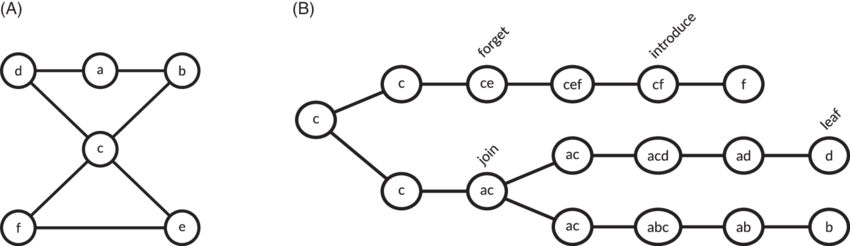
\includegraphics[width=0.95\textwidth]{./assets/nice_tree_decomposition}
	\end{center}
	\caption[Nice tree decomposition]{
		An example of a~nice tree decomposition with width three.
		On the~left, you can see the~decomposed graph,
		on the~right, a~nice tree decomposition
		with \LeafNode{}s on the~right and the~\RootNode{} on the~left.
		Figure inspired by~\cite{nice_tree_decomposition_img}.
	}%
	\label{fig:nice_tree_decomposition}
\end{figure}

An example of a nice tree decomposition with bags showed in~vertices
is shown in~\cref{fig:nice_tree_decomposition}.
%
Note that a~vertex \( v \in V(G) \) can be introduced multiple times
(in multiple branches of \( T \)),
but forgotten only once.
%
Otherwise, there must be an~\IntroduceVertexNode{} above a~\ForgetVertexNode{} in~\( T \).
But then there are multiple subgraphs in~\( T \)
such that \( v \) is in~their every bag.
This does not fulfill the~definition of a~tree decomposition.

By \( V_t, t \in T \), we~denote the~set of vertices introduced by \( t \)
and all its child nodes.
%
\begin{lemma}[\cite{book_parametrized_algorithms}]
	Any tree decomposition of width at~most \( k \) can be converted to
	a~nice tree decomposition of width at~most \( k \)
	in time \( O(k^2 \cdot \max(|V(T)|, |V(G)|)) \).
	The~nice decomposition tree has at~most \( O(k|V(G)|) \) nodes.
\end{lemma}

The~problem of finding treewidth is NP-complete~\cite{tree_width_np_complete}.
Luckily, the~problem is studied a~lot and
there exist efficient approximation algorithms~\cite{tree_width_approximation}.
We~consider nice tree decompositions as given along with a~graph
and do not consider runtime required to find it.

In~\IntroduceVertexNode{} introducing \( v \), all the~edges incident to \( v \)
to vertices in~\( X_{t'} \) are usually considered while processing \( t \).
%
For~some problems, it~is beneficial to divide this operation further.
First, a~vertex \( v \) is introduced with no edges using a~\IntroduceVertexNode{},
and later all the~edges corresponding to the~vertex are introduced using new \IntroduceEdgeNode{}s
just before one of its vertices is forgotten.

We~define an~edge bag \( Y_t \subseteq E(G), t \in T \) similarly as vertex bags \( X_t \).
%
Let~\( t' \) be a~direct ancestor of~\( t \).
For~\IntroduceVertexNode{}, we~define \( Y_t = Y_{t'} \).
For~\ForgetVertexNode{} forgetting vertex \( v \),
the following condition holds: \( Y_t = Y_{t'} \setminus \{ e \in E(G) \mid v \in e\} \).
%
\begin{definition}[\IntroduceEdgeNode{}~\cite{book_parametrized_algorithms}]
	An~\IntroduceEdgeNode{} node \( t \in T \) is a~node
	labeled with an~edge \( e = \{u, v\} \in E(G) \)
	such that \( u, v \in X_t \) and with exactly one child \( t' \)
	such that \( X_t = X_{t'} \), \( Y_t \setminus Y_{t'} = \{e\} \).
	We~say that \( e \) is \emph{introduced} by \( t \).
	Each edge can be introduced at~most once in~\( T \).
\end{definition}
%
By \( E_t, t \in T \), we~denote the~set of edges introduced by \( t \)
and all its child nodes.
By \( G_t, t \in T \), we~mean the~graph \( G_t = (V_t, E_t) \).

For~edge \( \{u, v\} \in E(G) \), we~can transform a~nice tree decomposition \( T \)
by adding \IntroduceEdgeNode{}s \( t \) above \IntroduceVertexNode{}s of \( u, v \)
and bellow \ForgetVertexNode{}s of \( u, v \in T \).
%
W.l.o.g., suppose that the~\ForgetVertexNode{}~\( t_v \) of \( v \) is
an~ancestor of the~\ForgetVertexNode{}~\( t_u \) of \( u \in T \).
Let~\( t_c \) be the~only child of \( t_u \).
%
We~add \IntroduceEdgeNode{}~\( t_e \) for~edge \( \{u, v\} \)
as a~direct child of \( t_u \) and make \( t_c \) the~direct child of \( t_e \).
%
We~can update a~nice tree decomposition by doing
a~top-down tree traversal and adding \IntroduceEdgeNode{}s for~all edges.
The~transformation requires \( O(nk) \) time (as the~number of edges is bounded by \( nk \)).
From now on, we~refer only to these transformed nice tree decompositions.

%
\begin{observation}
	\label[observation]{observ:no_edges_in_nodes}
	%
	The~edge bag of each node except for~\IntroduceEdgeNode{}s
	in a (transformed) nice tree decomposition \( t \in T \) is empty.
\end{observation}
%
This can be seen that the~edges are added right before one of the~vertices
they are incident to is forgotten. \ForgetVertexNode{} removes all the~edges
that are incident to the~forgotten vertex.

%%%%%%%%%%%%%%%%%%%%%%%%%%%%%%%%%%%%%%%%%%%%%%%%%%%%%%%%%%%%%%%%%%%%%%%%%%%%%%%%
\section{Monadic second-order logic}

Monadic second-order logic~(\MSO{}) on graphs is a~logical system based on
well-known predicate logic.
In~the~world of parameterized algorithms,
it~often comes handy --- if~we are able to represent a~problem using~\MSO{},
then there exists an~FPT algorithm parameterized by treewidth
that can solve the~problem~\cite{tree_width_mso}.

\subsection{Introduction to \( \text{MSO}_2 \)}

In~the~following paragraphs we~paraphrase and simplify formal definition
from~\cite{book_parametrized_algorithms}.
We~presume that the reader is already familiar with first-order predicate logic.
Second-order predicate logic as an~extension of first-order predicate logic,
that adds option to quantify over predicates.

\MSO{}~is realization of second-order predicate logic%
\nohznamka{
	We~need second-order logic as quantification over subsets of vertices or edges
	corresponds to quantification over predicates defining the~subsets.
	Without this requirement, we~could talk
	about the~monadic first-order logic \( \text{MSO}_1 \).
}.
Formulas can be formed from
variables, constants, predicates,
boolean operations \( \lnot, \land, \lor, \Rightarrow, \Leftrightarrow \)
and quantifiers \( \forall, \exists \).
Complex formulas are created recursively from atomic formulas
by applying schema related to each operation or quantifier.
This process is the~same as in~the~first-order predicate logic.

Formulas of \MSO{} can use four types of variables:
single vertices, single edges, subsets of vertices, and subsets of edges.
%
An~application of a~graph~\( G \) to a~formula~\( \phi \) is called \emph{evaluation}
of \( \phi \) in~\( G \).
This represents the~process of assigning values from \( G \) to variables in~\( \phi \).
%
By \( u^G \) we~denote evaluation of variable \( u \) in~graph~\( G \).
%
A~\emph{free variable} is a~variable such that it~is not quantified by any predicate.
Let~\( \Sigma \) denote all free variables of \( \phi \).
%
Let~\( \Sigma^G \) be a~sequence of evaluations for each variable in~\( \Sigma \).
Tuple \( \langle G, \Sigma^G \rangle \) is called the~\emph{structure}
in~which \( \phi \) is evaluated.
If~\( \phi \) is true in~\( \langle G, \Sigma^G \rangle \),
then \( \langle G, \Sigma^G \rangle \)
is called a~\emph{model} of \( \phi \)~\cite{book_parametrized_algorithms}.
%
To form atomic formulas in~\MSO{}, we~allow only the following base predicates:
%
\begin{itemize}
	\item For~\( u \) representing a~vertex (edge) variable
	      and \( X \) is a~vertex (edge) subset,
	      we~can write formula~\( u \in X \).
	      For~\( G \), the~formula is true if~\( u^G \in X^G \) is true.
	\item Let~\( u \) be a~vertex variable and \( e \) be an~edge variable,
	      then we~can write formula~\( \inc (u, e) \).
	      For~\( G \), the~formula is true if~\( u^G \) is an~endpoint of \( e^G \).
	\item For~any two variables \( u, v \) of the~same type, we~can write \( u = v \).
	      For~\( G \), the~formula is true if~\( u^G = v^G \).
\end{itemize}
%
We~also allow simplifications like \( \ne, \not\in \).
As obvious from types of variables, we~can quantify over vertices, edges,
subsets of vertices and subsets of edges.

It~is beneficial to define auxiliary predicates to simplify our work.
We~show examples taken from~\cite{book_parametrized_algorithms}.
First, we~show predicate \( \text{adj} \) represents if~two vertices are adjacent.
%
\begin{align*}
	\text{adj}(u, v) \coloneqq (u \ne v) \land (\exists e \in E : \inc (u, e) \land \inc (v, e))
\end{align*}
%
For~a~graph \( G = (V, E) \), we~can represent the connectivity of its induced subgraph
on vertices \( X \subseteq V \) with the~following predicate~\cite{book_parametrized_algorithms}.
%
\begin{align*}
	\text{connected}(X) \coloneqq \, &
	\forall Y \subseteq V : \Big(
	(
	\exists u \in X : u \in Y \land
	\exists v \in X : v \not\in Y
	)
	\\ &
	\Rightarrow
	(
	\exists u, v \in X : \text{adj}(u, v) \land u \in Y \land v \not\in Y
	)\Big).
\end{align*}
%
Notice that we~used our previously defined predicate as an~alias.
For~\( X = V \), the~formula would read as:
``For each separation of a~graph, there exists an~edge connecting both partitions''.

\subsection{Relation to treewidth}

In~the following, for~a~formula~\( \phi \) by \( \|\phi\| \)
we~denote the~length of the~encoding of \( \phi \) as a~string.
%
\begin{theorem}[Courcelle's theorem,~\cite{tree_width_mso,book_parametrized_algorithms}]%
	\label{theorem:courcelles_theorem}%
	Assume that \( \phi \) is a~formula of \MSO{} and
	\( G \) is an~\( n \)-vertex graph equipped
	with evaluation of all the~free variables of \( \phi \).
	Suppose, moreover, that a~tree decomposition of \( G \) of width \( k \) is provided.
	Then there exists an~algorithm that verifies whether \( \phi \)
	is satisfied in~\( G \) in~time \( f (\|\phi\|, k) \cdot n \),
	for some computable function \( f \).
\end{theorem}
%
If~we are given an~optimal tree decomposition, or we~manage to find good enough
approximation, we~know that we~can decide any formula in~\MSO{} in~a~time
polynomial in~\( n \), but we~are given no guaranties for~the~complexity~of~\( f \).

\subsection{Expressing NAC-colorings using \( \text{MSO}_2 \)}

In~this section, we~present results from our previous paper~\cite{my_paper}.
By \( V \) we~denote the~set of all vertices and
by \( E \) the~set of all edges.
We~start by defining other auxiliary predicates:
%
\begin{itemize}
	\item For~a~subset of edges \( F \), we~define predicate
	      %
	      \begin{align*}
		      \text{deg2}(F) \coloneqq \predsp
		       & \forall e \in F \predsp \forall v \in V : \inc (v, e) \Rightarrow                                                                      \\
		       & \exists e' \in F \setminus \{e\} : \Big( \inc (v, e') \land \big(\forall e'' \in F \setminus \{e, e'\}: \lnot \inc (v, e'')\big)\!\Big).
	      \end{align*}
	      %
	      The~predicate says that all vertices incident to edges in~\( F \) have degree two.
	      %
	\item For~a~subset of vertices \( U \) and a~subset of edges \( F \), we~define predicate
	      %
	      \begin{align*}
		      \text{incident}(U, F) \coloneqq \predsp
		       & \big(\forall v \in U \predsp \exists e \in F : \inc (v, e)\big)                                                       \\
		       & \land \big(\forall e \in F \predsp \exists v_1, v_2 \in U : v_1 \ne v_2 \land \inc (v_1, e) \land \inc (v_2, e)\big).
	      \end{align*}
	      %
	      The~predicate says that \( U \) are vertices of the~subgraph induced by \( F \)
	      and that \( F \) are edges of the~subgraph induced by \( U \),
	      e.g. \( (U, F) \) is an~induced subgraph of \( (V, E) \).
	      %
	\item For~a~subset of edges \( F \), we~define predicate
	      %
	      \begin{align*}
		      \text{cycle}(F) \coloneqq \predsp
		      \big( \exists X \subseteq V : \text{incident}(X, F) \land \text{connected}(X) \big)
		      \land \text{deg2}(F).
	      \end{align*}
	      %
	      The~predicate says that edges \( F \) form a~cycle.
	      %
	\item For~subsets of edges \( F_1, F_2 \), we~define predicate
	      %
	      \begin{align*}
		      \text{partition}(F_1, F_2) \coloneqq \predsp
		       & (\exists e_1, e_2 \in E : e_1 \in F_1 \land e_2 \in F_2 )    \\
		       & \land (\forall e \in E : e \in F_1 \lor e \in F_2 )          \\
		       & \land (\forall e \in E : e \not\in F_1 \lor e \not\in F_2 ).
	      \end{align*}
	      %
	      The~formula reads as: ``Both the~partitions are not empty,
	      and each edge is in~exactly one of the~partitions''.
	\item For~subsets of edges \( C, F_\red, F_\blue \), we~define predicate
	      %
	      \begin{align*}
		      \text{NACcond}(C, F_\red, F_\blue) \coloneqq \predsp
		       & C \subseteq F_\red \lor C \subseteq F_\red
		      \\
		       & \lor (\exists e_1, e_2, e_3, e_4 \in E :
		      e_1 \ne e_2 \land e_3 \ne e_4
		      \\
		       & \qquad \land e_1, e_2 \in F_\red \land e_3, e_4 \in F_\blue ).
	      \end{align*}
	      %
	      The~predicate says that the~cycles \( C \) is not an~almost cycle.
	      %
\end{itemize}
%

With the~predicates ready, we~can proceed to the~theorem.
%
\begin{theorem}[\cite{my_paper}]
	The~problem of existence of a~NAC-coloring is fixed-parameter
	tractable when parameterized by treewidth.
\end{theorem}
%
\begin{proof}
	We~can express the~NAC-coloring problem
	as a~formula~\( \phi \) in~\MSO{} as follows:
	%
	\begin{align*}
		\exists E_\red, E_\blue \subseteq E : \,
		 & \text{partition}(E_\red, E_\blue)                                                                 \\
		 & \land \big(\forall C \subseteq E : \text{cycle}(C) \land \text{NACcond}(C, E_\red, E_\blue) \big)
		.
	\end{align*}
	%
	By \Cref{theorem:courcelles_theorem},
	there exists an~FPT algorithm parameterized by treewidth
	that can resolve \( \phi \) and therefore resolve the~question whenever a~graph has a~NAC-coloring.
\end{proof}
%
The~proof shows us that there exists such an~algorithm,
but it~does not give us explicit steps to follow
(even tough they can be deduced from the~original proof of \Cref{theorem:courcelles_theorem}).
Still, the~complexity guaranties of the~algorithm are not very clear.
In~the~following section, we~define our
own FPT algorithm that solves the~NAC-coloring problem
while not relying on~\MSO{}.



\section{FPT algorithm}

In~this section, we~first introduce the~core idea of
our FPT algorithm for~NAC-coloring counting,
define a~cache function,
show and prove the~recursive formulas for~the~cache function for each node in~a~tree decomposition
and determine the~complexity of the~algorithm.
% Lastly, we~propose optimizations to the~algorithm by also empowering monochromatic classes.
We propose two approaches, one using \IntroduceEdgeNode{}s and one using \IntroduceVertexWithEdgesNode{}s.
Lastly, we~ discuss how a~certificate can be obtained
and propose additional optimizations to the~algorithm.


\subsection{The algorithm}

Our algorithm is slightly similar to Steiner tree search algorithm
as described in~\cite{book_parametrized_algorithms} as both the~problems require connectivity
among vertex partitions. Unlike in~the~Steiner tree search algorithm,
our state space is even larger and all the~state mapping operations are significantly different.

Before we~start, we~define some terms that come useful later.
When we~talk about a~component, we~mean a~connected component.
%
\begin{definition}[Connector, Neighboring components]
	For~a~graph \( G \) with a~\rbcol{} \( \gamma \)
	and two distinct components of \( G[\Ered] \), resp.\ \( G[\Eblue] \),
	with vertex sets \( U_1 \) and \( U_2 \),
	a~\emph{connector} is an~edge \( e = \{u_1, u_2\} \in E(G) \)
	such that \( u_1 \in U_1 \) and \( u_2 \in U_2 \).
	%
	The~components are \emph{neighboring} if~there exists
	a~connector for~these two components.
\end{definition}
%

First, we~want to build the~intuition for~the~upcoming operations.
Let~us have a~graph \( G \) and all NAC-colorings of the~graph \( \nac{G} \).
Let~us add an~edge \( e = \{u, v\}, e \not\in E(G) \) to form the~graph~\( G' \).
We~want to obtain~\( \nac{G'} \) based on \( \nac{G} \).
%
Let~us have \( \delta \in \nac{G} \),
we~want to extend it~to \( \delta' \) where w.l.o.g.\ \( \delta'(e) = \blue \).
Coloring \( \delta' \) is a~NAC-coloring unless an~almost cycle is formed in~\( G' \).
In~that case, one of the~following cases must be true:
%
\begin{itemize}
	\item Both vertices \( u, v \) are in~the~same component in~\( G[\Ered] \).
	      An~almost cycle is formed
	      from \( \red \) \( u \)-\( v \)-path in~the~component
	      and edge \( e \) with \( \blue \) color.
	\item Vertices \( u, v \) lay in~neighboring components in~\( G[\Eblue] \)
	      i.e.\ there is a~\( \red \) connector between the~components.
	      An~almost cycle is formed from \( \blue \) paths in~each component,
	      the~\( \red \) connector and \( \blue \) edge \( e \).
\end{itemize}
%
In~all other cases, an~almost cycle cannot be formed by adding a~\( \blue \) edge \( e \).
Note that a~vertex cannot be in~multiple components for~the~given color
as this fact would mean that the~components are not maximal.

To create \( \nac{G'} \), we~extend the~colorings
in~\( \nac{G} \cup \{ \delta_\red \} \), where \( \delta_\red \)
colors all edges in~\( G \) with \( \red \) color.
We~do the~whole checking process likewise
for~\( e \) colored \( \red \) --- all the~colors used get swapped.
Then we~keep only the~surjective colorings that did not form an~almost cycle.

We~define an~\emph{almost NAC-coloring}
as a~\rbcol{} such that there are no almost cycles formed.
The~conditions are the~same as for~NAC-coloring
except that the~surjectivity requirement is dropped.
By \( \anac{G} \), we~denote the~set of all almost NAC-colorings of \( G \).
We~use the~notion of almost NAC-coloring for~the~rest of the~section.
Later when output is read in~a~\RootNode{},
based on the~number of all almost NAC-colorings of~\( G \)
the~number of all NAC-colorings of~\( G \) is obtained.
Note that a~graph with no edges has no almost NAC-colorings.

We~use \emph{dynamic programming}, a~well-known technique for~solving problems
where the~problem can be subdivided into smaller subproblems.
Usually, some base cases are solved trivially and then a~subproblem
is solved based on the~solution of its smaller subproblems.
%
Often it~is a~case that a~smaller subproblem would be solved multiple times
as it~is a~part of multiple larger subproblems.
Its first result is therefore cached and reused,
reducing the~total running time significantly.
%
In~other cases like ours, it~is a~common approach for~traversing
some data structure like matrix or a~tree.
%
There are many popular dynamic programming algorithms
like \textsc{Edit Distance}, \textsc{Matrix Chain Multiplication} or \textsc{Longest Common Subsequence}.

In~the~following sections,
we~work with a~nice tree decomposition \( T \) of width \( k \)
of a~graph \( G \).
%
We~define a~state space \( S \) of \emph{states}
that will be used by our cache in~our dynamic programming algorithm.
We~denote all partitions of a~nonempty set \( X \) by \( \mathcal{F}(X) \),
and we~put \( \emptyset = \mathcal{F}(\emptyset) \).

%
\begin{definition}[State space]
	Let~\( t \in T \) be a~node in~the~nice tree decomposition tree and
	\( X_t \) be its bag of vertices.
	%
	A~\emph{state} is formed by a~tuple \( s = (P_\red, R_\red, P_\blue, R_\blue) \)
	where \( P_\red, P_\blue \in \mathcal{F}(X_t)\) are partitions of \( X_t \),
	and \( R_\red\), resp.\ \(R_\blue \), is a~symmetric irreflexive relation
	on parts in~\( P_\red\), resp.\ \(P_\blue \).
	%
	All such states on \( X_t \) form the~\emph{state space} \( S_t \).
\end{definition}
%
For~some \( t \in T \), a~\rbcol{} \( \gamma \) of \( G_t \)
is \emph{consistent} with a~state \( s_t = (P_\red, R_\red, P_\blue, R_\blue) \in S_t \)
if~\( \red \) and \( \blue \) components of \( \gamma \) form \( P_\red \) and \( P_\blue \)
when \( u, v \in X_t \) are in~the~same part in~\( P_\red \) or \( P_\blue \)
if~and only if~they are in~the~same \( \red \) or \( \blue \) component induced by \( \gamma \).
There are connectors between two components if~and only if
the~corresponding parts are in~relation \( R_\red \) or \( R_\blue \).
%
Note that we~define consistence for~general \rbcol{}s,
but usually we~use them with almost NAC-colorings only.
%
Two parts are \emph{neighboring} if~their corresponding components are neighboring.
When we~talk about \emph{\( \red \) half of a~state},
we~mean \( P_\red \) and \( R_\red \),
analogically for~\( \blue \).
%
Note that the~state space is somewhat large.
We~elaborate on the~size in~the~proof of~\Cref{thm:fpt_algo}.
%
\begin{observation}
	For each \rbcol{} \( \gamma \) on \( G_t \),
	there is a single state \( s \in S_t \) consistent with it.
	Multiple \rbcol{} can be consistent with a~single state.
\end{observation}
%

In~a~dynamic programming algorithms, a~cache function is gradually computed
from the~simplest subproblems to the~largest ones.
Here, we~have a~function that already has all the~values computed,
and we~show relations for~neighboring nodes in~\( T \).
There recursive relations can be then used in~an~implementation.
%
\begin{definition}[Cache function]
	For~a~nice tree decomposition \( (T, \{X_t\}) \) on a~graph \( G \),
	a~\emph{cache function} \( c: \mathcal{S} \to \N_0 \)
	where \( \mathcal{S} = \{ (t,s): t \in T \in S_t \} \)
	is the~function that maps \( (t, s) \)
	to the~number of almost NAC-colorings of \( G_t \) consistent with \( s \).
\end{definition}
%
For~the~following definitions, lemmas, proofs and theorems, let~us fix
a~nice tree decomposition \( T \) of a~graph \( G \) and width \( k \)
and a~cache function \( c \) on \( T \).
%
\begin{lemma}%
	\label[lemma]{lemma:state_space_sum}
	%
	For~\( t \in T \) and a~graph \( G_t \),
	% the following condition holds:
	\( |\anac{G_t}| =  \sum_{s \in S_t} c[t, s] \).
\end{lemma}
%
\begin{proof}
	%
	For each~\( \delta \in \anac{G_t} \),
	there is a~single state \( s \in S_t \) consistent with~\( \delta \).
	Therefore, if~we sum over all states \( s \in S_t \),
	we consider every~\( \delta \in \anac{G_t} \) and get \( |\anac{G_t}| \).
\end{proof}
%
\begin{observation}
	For~two nodes \( t_1, t_2 \in T \) such that \( G_{t_1}, G_{t_2} \)
	are isomorphic up to isolated vertices,
	then for~bags \( X_{t_1}, X_{t_2} \) and state spaces \( S_{t_t}, S_{t_2} \),
	it holds that \( \sum_{s \in S_{t_1}} c[t_1, s] = \sum_{s \in S_{t_2}} c[t_2, s] \).
\end{observation}
%
% \begin{proof}
% 	Isolated vertices are not important for~almost NAC-colorings
% 	as we~consider edges only.
% 	Therefore, as \( |\anac{G_{t_1}}| = |\anac{G_{t_2}}| \),
% 	by \Cref{lemma:state_space_sum}
% 	it holds that \( \sum_{s \in S_{t_1}} c[t_1, s] = \sum_{s \in S_{t_2}} c[t_2, s] \).
% \end{proof}
%

In~the~following lemmas, we~show recursive relations for~\( c \) that must hold
for~neighboring nodes in~\( T \).
%
In~the~following proofs,
we~often describe states that cannot be consistent with
any almost NAC-colorings and hence have zero value in~\( c \).

We~prove the correctness of our algorithms by induction.
The~base case is for~\LeafNode{}s, for~other nodes we~split the~reasoning for~cases where
there is or is not at~least one edge in~\( G_t \).
%
Following lemmas always show mapping from child node \( t' \) states \( S_{t'} \)
to parent node \( t \) states \( S_t \).
We~extend almost NAC-colorings on \( G_{t'} \) and
map which states in~\( S_{t'} \) map to which state in~\( S_t \)
or produce an~almost cycle when extended.
%
For~a~color \( a \in \{\red, \blue\} \),
we~define \( \bar{a} \) to be the~opposite color.

%%%%%%%%%%%%%%%%%%%%%%%%%%%%%%%%%%%%%%%%%%%%%%%%%%%%%%%%%%%%%%%%%%%%%%%%%%%%%%%%
% Leaf node
%%%%%%%%%%%%%%%%%%%%%%%%%%%%%%%%%%%%%%%%%%%%%%%%%%%%%%%%%%%%%%%%%%%%%%%%%%%%%%%%
\subsubsection*{\LeafNode{}}

\begin{lemma}%
	\label[lemma]{lemma:fpt_leaf_node}
	%
	Let~us have a~\LeafNode{} \( t \in T \).
	It~holds that \( c[t, s] = 0 \) for~all \( s \in S_t \).
\end{lemma}
%
\begin{proof}
	There are no edges in~\( G_t \) as there are no vertices
	neither in~\( X_t \) nor \( V_t \).
	By definition of the~cache function,
	\( c \) must hold zero for each state of a~\LeafNode{}.
\end{proof}
%
Note that for~a~\LeafNode{} \( t \in T \),
the~only state in~\( S_t \) is \( (\emptyset, \emptyset, \emptyset, \emptyset) \)
as \( X_t = \emptyset \).

%%%%%%%%%%%%%%%%%%%%%%%%%%%%%%%%%%%%%%%%%%%%%%%%%%%%%%%%%%%%%%%%%%%%%%%%%%%%%%%%
% Introduce Vertex Node
%%%%%%%%%%%%%%%%%%%%%%%%%%%%%%%%%%%%%%%%%%%%%%%%%%%%%%%%%%%%%%%%%%%%%%%%%%%%%%%%
\clearpage
\subsubsection*{\IntroduceVertexNode{}}

\begin{lemma}%
	\label[lemma]{lemma:fpt_introduce_vertex_node}
	%
	Let~an~\IntroduceVertexNode{} \( t \in T \) be
	the~only parent of \( t' \in T \).
	Let~\( v \) be the~only vertex in~\( X_t \setminus X_{t'} \).
	%
	If~there is no edge in~the~graph \( G_t \), then \( c[t, s] = 0 \) for each \( s \in S_t \).
	%
	Otherwise, the~cache function \( c \) satisfies for
	\( s=(P_\red, R_\red, P_\blue, R_\blue) \in S_t \) the~following:
	%
	\begin{align*}
		c[t, s] & =
		\begin{cases}
			0,         & \text{if } \exists a \in \{\red, \blue\} : \{v\} \not\in P_a,                    \\
			0,         & \text{if } \exists a \in \{\red, \blue\} \exists p \in P_a : (\{v\}, p) \in R_a, \\
			c[t', s'], & \text{otherwise},
		\end{cases}
	\end{align*}
	where
	\begin{align*}
		s' & \coloneqq (P_\red \setminus \{\{v\}\}, R_\red, P_\blue \setminus \{\{v\}\}, R_\blue).
	\end{align*}
\end{lemma}
%
The~state \( s' \) represents the~state where \( v \) is not present in~any part
and where the~same parts stay neighbors as in~\( s \).
%
\begin{proof}
	By definition, there are no almost NAC-colorings
	in~\( G_t \) if~\( G_t \) has no edges,
	therefore \( c[t, s] = 0 \) for each \( s \in S_t \).
	%
	Otherwise, if~a vertex \( v \) is in~a~part of \( P_\red \) or \( P_\blue \) with other vertices,
	the~cache function must be zero as \( v \) is an~isolated vertex in~\( G_t \)
	and therefore no almost NAC-coloring consistent with such state exists.
	Otherwise, there must be a~part \( \{v\} \).
	%
	Also, as \( v \) is an~isolated vertex in~\( G_t \), there cannot be a~connector
	connecting this and another component.
	Thus, for~all states where there exists
	a~part neighboring \( \{v\} \), there are no consistent almost NAC-colorings
	and therefore the~cache function must be also zero.
	%
	For~an~almost NAC-coloring \( \delta \) on \( G_{t'} \) consistent with
	a~state \( s' \in S_{t'} \),
	by adding part \( \{v\} \) to \( P_\red' \) and \( P_\blue' \)
	we get some \( s \in S_t \) that is also consistent with \( \delta \) in~\( G_t \).
	Adding and removing part \( \{v\} \) is a~bijective operation in~this context.
	Therefore, \( c[t, s] = c[t', s'] \) holds for~all states.
	%
	We~have \( anac{G_t} = anac{G_{t'}} \) since \( E(G_t) = E(G_{t'}) \).
	Each almost NAC-coloring is consistent
	with \( s \) and \( s' \) given as described.
\end{proof}
%
To summarize, values from child node are propagated to the~states
where \( v \) is added and stays isolated.

%%%%%%%%%%%%%%%%%%%%%%%%%%%%%%%%%%%%%%%%%%%%%%%%%%%%%%%%%%%%%%%%%%%%%%%%%%%%%%%%
% Forget Vertex Node
%%%%%%%%%%%%%%%%%%%%%%%%%%%%%%%%%%%%%%%%%%%%%%%%%%%%%%%%%%%%%%%%%%%%%%%%%%%%%%%%
\subsubsection*{\ForgetVertexNode{}}

\begin{lemma}%
	\label[lemma]{lemma:fpt_forget_vertex_node}
	%
	Let~a~\ForgetVertexNode{} \( t \in T \) be
	the~only parent of \( t' \in T \).
	Let~\( v \) be the~only vertex in~\( X_{t'} \setminus X_t \).
	%
	If~there are no edges in~the~graph~\( G_t \),
	then \( c[t, s] = 0 \) for each \( s \in S_t \).

	Otherwise, the~cache function for~\( s=(P_\red, R_\red, P_\blue, R_\blue) \in S_t \)
	satisfies that:
	%
	\begin{align*}
		c[t, s] & = \sum_{s' \in S'} c[t', s'],
	\end{align*}
	where for~\( a \in \{\red, \blue\} \)
	\begin{align*}
		d(p)               & \coloneqq p \setminus \{v\},                                                                                   \\
		D(P)               & \coloneqq \{d(p) \mid p \in P \} \setminus \{\emptyset\},                                                      \\
		\mathcal{P'}_a     & \coloneqq \{ P_a' \in \mathcal{F}(X_{t'}) \mid D(P_a') = P_a \},                                               \\
		\mathcal{R'}(P_a') & \coloneqq \{ R_a' \subseteq P_a' \times P_a' \mid \forall (p_1, p_2) \in R_a' :                                \\
		                   & \qquad (d(p_1), d(p_2)) \in R_a \lor d(p_1) = \emptyset \lor d(p_2) = \emptyset \},                            \\
		S'                 & \coloneqq \{(P_\red', R_\red', P_\blue', R_\blue') \mid P_a' \in \mathcal{P'}_a, R' \in \mathcal{R'}(P_a') \}.
	\end{align*}
\end{lemma}
%
Recall that \( R_\red, R_\blue \) are relations --- sets of pairs.
By \( d(p) \) we~denote deletion of the~vertex \( v \) from a~part \( p \),
and by \( D(P) \) we~denote deleting the~vertex \( v \) from all the~parts in~partition \( P \)
--- if~\( \{v\} \in P \), \( \emptyset \) is also cleared.
Set \( \mathcal{P'}_a \) denotes all the~partitions
such that removing \( v \) from them gives \( P_a \).
Mapping \( \mathcal{R'}(P_a') \) denotes all the~relations \( R_a' \)
for~\( P_a' \in \mathcal{P'}_a \) that correspond with \( R_a \) when \( v \) is removed
--- parts are updated or relations to \( \{v\} \) is removed.
States \( S' \subseteq S_{t'} \) is the~set of all states that
correspond to state \( s \) when \( v \) is removed.
%
\begin{proof}
	If~there are no edges in~\( G_t \), none are added by a~\ForgetVertexNode{}.
	Therefore, \( c[t, s] = 0 \) for~all \( s \in S_t \).
	%
	Otherwise, we~know that \( G_t = G_{t'} \).
	%
	For~\( s \in S_t \),
	let us have an~almost NAC-coloring \( \delta \) consistent with \( s \).
	We~show all states in~\( S_{t'} \) that may be consistent with \( \delta \).
	We~show how w.l.o.g.\ \( \blue \) half of \( s' \in S_{t'} \) looks
	based on \( \blue \) half of \( s \).

	Let~\( v \) be in~a~\( \blue \) component \( C \) such that
	\( C \) corresponds to no part in~\( P_\blue \).
	Then for~\( s' \) it~holds that \( \{v\} \in P_\blue' \).
	%
	Components neighboring in~\( R_\blue \)
	are also neighboring in~\( R_\blue' \), therefore \( R_\blue \subseteq R_\blue' \).
	%
	Component \( C \) may be neighboring with
	components corresponding to parts in~\( P_\blue' \).
	% It~cannot be specified with witch without deeper knowledge about \( \delta \),
	% hence we~consider all possible relations.
	To cover all possible \( \delta \),
	we consider all possible relations \( R_\blue' \).

	Now let~\( v \) in~a~component corresponding to a~part \( p \in P_\blue \).
	Then part in~\( P_\blue' \) correspond to the~same components and the~only
	change is that part \( p \) is replaced by \( p \cup \{v\} \).
	Neighboring relation is updated accordingly.

	By this we~described \( \red \) and \( \blue \) halves of states in~\( S_{t'} \)
	such that they are consistent with the~same almost NAC-colorings as \( s \).
	We~used exactly the~same operations as in~the~statement of the~lemma.

	When we~consider all states in~\( S_t \), we~cover all almost NAC-colorings on \( G_t \)
	and hence also all states in~\( S_{t'} \) must get \( s \in S_t \) to map to.

	%%%%%%%%%%%%%%%%%%%%%%%%%%%%%%%%%%%%%%%%%%
	% Old proof left for~nostalgia reasons
	%%%%%%%%%%%%%%%%%%%%%%%%%%%%%%%%%%%%%%%%%%
	% Let~us have \( \delta \in \anac{G_{t'}} \)
	% and a~consistent state \( s' \in S_{t'} \).
	% In~\( G_t \), \( \delta \) is consistent with a~state \( s \in S_t \).
	% Note that components in~\( G_t \) and \( G_{t'} \) are the~same.
	% %
	% We~now describe how w.l.o.g.\ \( \blue \) half of \( s \) looks
	% based on the~\( \blue \) half of \( s' \).
	% The~halves do not influence ech other here.
	% %
	% If~\( \{v\} \) is a~part in~\( P_\blue' \),
	% it~is no longer considered in~\( P_\blue \),
	% therefore \( P_\blue' \setminus \{\{v\}\} = P_\blue \).
	% All pairs with \( \{v\} \) are removed from \( R_\blue' \).
	% %
	% If~\( \{v\} \) is not a~part in~\( P_\blue' \),
	% \( v \) is in~another part of \( P_\blue' \).
	% In~\( P_\blue \), the~parts look the~same except they do not
	% contain~\( v \). Relation \( R_\blue' \) is updated analogically.
	% %
	% Either of these statements hold for~the~\( \blue \) half,
	% analogically for~the~\( \red \) half.
	% %
	% The~mappings we~prove are exactly \( \mathcal{P'} \) and \( \mathcal{R'} \)
	% in~the~statement of the~lemma.
	% %
	% We~showed mapping for each \( s' \in S_{t'} \) into \( S_t \).
	% %
\end{proof}
%

%%%%%%%%%%%%%%%%%%%%%%%%%%%%%%%%%%%%%%%%%%%%%%%%%%%%%%%%%%%%%%%%%%%%%%%%%%%%%%%%
% Introduce Edge Node
%%%%%%%%%%%%%%%%%%%%%%%%%%%%%%%%%%%%%%%%%%%%%%%%%%%%%%%%%%%%%%%%%%%%%%%%%%%%%%%%
\subsubsection*{\IntroduceEdgeNode{}}

When discussing \IntroduceEdgeNode{} introducing edge \( e \),
we~first describe states in~\( S_{t} \)
that cannot be consistent with any almost NAC-coloring in~\( G_t \).
If~they can, we~call them \emph{allowed}, otherwise they are \emph{not allowed}.
Similarly, we~define this notion for~halves of a~state.
%
An~edge \emph{lies} in~a~part if~both its endpoints are in~the~part.
An~edge \emph{connects} two parts if~its endpoints are each in~one~part.
%
We~state conditions for~extending almost NAC-coloring \( \delta' \)
consistent with \( s' \in S_{t'} \)
by an~edge colored by one color first,
w.l.o.g.\ let~the~introduced edge \( e \) be colored \( \blue \).
%
To avoid confusion, note that in~the~following statements we~assume
a~state \( s \in S_t \) after the~edge \( e \) is added, not a~state \( s' \in S_{t'} \).
%
We~first state conditions for~\( \blue \) half of a~state \( s \):
%
\begin{description}
	\item[Edge \( e \) lies in~a~\( \blue \) part]
	      In~this trivial case, an~almost cycle is not created in~\( \blue \) components.
	      This is \emph{\( \blue \)-allowed}.
	      %
	\item[Edge \( e \) connects two neighboring \( \blue \) parts]
	      This causes an~almost cycle to be created as
	      components corresponding to the~parts
	      are now a~single component.
	      Therefore, the~state \( s \) does not describe
	      the~actual state for~any almost NAC-coloring in~\( G_t \)
	      as there should be only a~single part, and therefore this is \emph{not allowed}.
	      %
	\item[Edge \( e \) connects two non-neighboring \( \blue \) parts]
	      This is \emph{not allowed} as both parts
	      are now using this \( \blue \) edge and should be one part.
\end{description}
%
Now we~state conditions for~\( \red \) half of a~state \( s \):
%
\begin{description}
	\item[Edge \( e \) lies in~a~\( \red \) part]
	      In~this case, an~almost cycle is trivially created
	      through the~\( \red \) component,
	      therefore, this is \emph{not allowed}.
	      %
	\item[Edge \( e \) connects two neighboring \( \red \) parts]
	      This is \emph{\( \blue \)-allowed} as \( e \) is a~connector and
	      therefore the~parts need to be neighboring.
	      %
	\item[Edge \( e \) connects two non-neighboring \( \red \) parts]
	      This state is \emph{not allowed} as both parts
	      are now neighboring as \( e \) is a~connector.
	      This is \emph{not allowed}.
\end{description}
%
The~same check is done analogically for~\( \red \)-allowed.
A~state is allowed if~both its halves are \( \red \)-allowed or
both the~halves are \( \blue \)-allowed.
Otherwise, a~state is not allowed.

\begin{lemma}%
	\label[lemma]{lemma:fpt_introduce_edge_node}
	%
	Let~us have an~\IntroduceEdgeNode{} \( t \in T \) that is
	the~only parent of \( t' \in T \).
	It~holds that \( X_t = X_{t'} \),
	let \( e = \{u, v\} \) be the~edge introduced by~\( t \), \( e \in Y_t \setminus Y_{t'} \).
	%
	If~there is only a~single edge \( e \) in~\( G_t \)
	(the just introduced edge~\( e \)) in~\( E_t \),
	for each state \( s = (P_\red, R_\red, P_\blue, R_\blue) \in S_t \),
	the~cache function satisfies that:
	\begin{align*}
		c[t, s] & =
		\begin{cases}
			1, & \text{if } \exists a \in \{\red, \blue\} :                                                 \\
			   & \{u\}, \{v\} \in P_a \land \{u, v\} \in P_{\bar{a}}                                        \\
			   & \land \, \{(\{u\}, \{v\}),(\{v\}, \{u\})\} = R_a \land R_{\bar{a}} = \emptyset             \\
			   & \land \, \forall z \in V_t \setminus \{u, v\} : \{z\} \in P_a \land \{z\} \in P_{\bar{a}}, \\
			0, & \text{otherwise}.
		\end{cases} \\
	\end{align*}
	%
	Otherwise, if~the~state \( s \) is not allowed, then \( c[t, s] = 0 \).
	%
	For~an~allowed state~\( s \),
	the~only states \( s' = (P_\red', R_\red', P_\blue', R_\blue') \in S_{t'} \),
	such that almost NAC-colorings consistent with \( s' \) are extended
	to almost NAC-colorings consistent with \( s \) by adding \( \blue \) edge \( e \),
	are the~states that fulfill these conditions for~their both halves:
	%
	\begin{description}
		\item[Edge lies in~a~\( \blue \) part of \( s \)]
		      There are two possibilities for~the~\( \blue \) half of a~state \( s' \).
		      %
		      The~first is condition that \( P_\blue = P_\blue' \)
		      and \( R_\blue = R_\blue' \) must hold.
		      %
		      The~other condition is that the~endpoints of \( e \)
		      must be in~different \( \blue \) parts \( p_1, p_2 \in P_\blue' \)
		      such that these parts are not neighboring, e.g.\ \( (p_1, p_2) \not\in R_\blue' \).
		      The~other parts are the~same as in~\( P_\blue \),
		      except for~part \( p = p_1 \cup p_2, p \in P_\blue \),
		      e.g.\ \( P_\blue' \setminus \{p_1, p_2\} = P_\blue \setminus \{p\} \).
		      \( R_\blue \) and \( R_\blue' \) must also match accordingly.
		      %
		      Either of the~conditions has to be fulfilled.

		      % First we~query the~previous cache state with
		      % the~same partition and neighbors state.
		      % Then we~also need to add states where
		      % both the~components were not neighbors as no almost cycle was created
		      % and both the~separate components
		      % are now joined into a~single component.
		      % We~denote \( \blue \) components of such state
		      % as \( P_\blue' \) and \( R_\blue' \).
		      % Note, that other relations between partitions need to match.
		      %
		\item[Edge connects two neighboring \( \red \) parts of \( s \)]
		      There are two possibilities for~the~\( \red \) half of a~state \( s' \).
		      %
		      The~first condition is that \( P_\red = P_\red' \)
		      and \( R_\red = R_\red' \) must hold.
		      %
		      Now, let~\( p_1, p_2 \in P_\red \) be the~\( \red \) parts
		      of end vertices of \( e \).
		      The~other condition is that \( P_\red = P_\red' \) and
		      \( R_\red \setminus \{(p_{1}, p_{2}), (p_{2}, p_{1})\} = R_\red' \) must hold.
		      %
		      Either of the~conditions has to be fulfilled.

		      % Result is a~sum of previous states with the~same partitioning as \( P_\red \),
		      % for~first query we~use \( R_\red \),
		      % and then we~add query of \( R'_\red = R_\red \setminus \{(c(u), c(v)), (c(v), c(u))\} \)
		      % (with the~neighbor constraint removed).
	\end{description}
	%
	There are four distinct states \( s_1', s_2', s_3', s_4' \in S_{t'} \)
	that fulfil these conditions, one for each condition combination.
	%
	We~define a~function \( c_\blue \) that represents
	the~number of all almost NAC-colorings
	consistent with state \( s \in S_t \) on \( G_t \)
	where \( e \) is colored \( \blue \).
	The~value for~\( c_\blue \) satisfies that:
	%
	\begin{align*}
		c_\blue[t, s] & = c[t', s_1'] + c[t', s_2'] + c[t', s_3'] + c[t', s_4'].
	\end{align*}
	%
	The~same holds for~\( \red \) analogously.
	Cache function satisfies that  \( c[t, s] = c_\red[t, s] + c_\blue[t, s] \).
\end{lemma}
%
\begin{proof}
	For~the~case when \( e \) is the~only edge,
	there are exactly two almost NAC-colorings on \( G_t \).
	The~states consistent with these colorings are \( s_\red \) and \( s_\blue \)
	such that if~\( u, v \) are in~the~same part in~\( P_\red \), resp.\ \( P_\blue \),
	there are parts \( \{u\}, \{v\} \) (singletons) in~\( P_\blue \), resp.\ \( P_\red \),
	as these vertices cannot be yet connected by \( \blue \), resp.\ \( \red \), edges.
	Edge \( e \) is a~connector, so there must be a~corresponding neighboring
	relation \( (\{u\}, \{v\}) \in R_\blue \), resp.\ \( R_\red \).
	Other states are not consistent with any almost NAC-colorings.
	This is exactly what we~describe in~the~lemma.

	Otherwise, only allowed states may have consistent almost NAC-colorings on \( G_t \).
	%
	For~an~almost NAC-coloring \( \delta' \) on \( G_{t'} \),
	by adding w.l.o.g.\ a~single \( \blue \) edge \( e \),
	it is either extended to an~almost NAC-coloring \( \delta \) on \( G_t \)
	or an~almost cycle is created.

	Let~\( f \) the~only edge with a~different color in~the~almost cycle.
	Let~\( f \) be colored \( \red \).
	Then there is a~\( \blue \) path connecting its endpoints using \( e \),
	as there was no such \( \blue \) path before.
	Therefore, there must be two \( \blue \) components \( p_1', p_2' \) in~\( G_{t'} \)
	connecting endpoints of \( e \) to \( f \).
	Hence, \( f \) must be a~connector connecting \( p_1' \) and \( p_2' \),
	and parts \( p_1' \) and \( p_2' \) are neighboring.
	But we~do not consider such states in~\( s_1', \dots, s_4' \).

	Let~us now consider \( f \) is colored \( \blue \).
	Then \( e = f \) and
	there must be a~\( \red \) path in~\( G_{t'} \) connecting its endpoints.
	This path must be in~a~single \( \red \) component corresponding
	to a~\( \red \) part \( p \in P_\red' \cap P_\red \).
	But we~do not consider such states in~\( s_1', \dots, s_4' \).

	Now we~show what a~state \( s \in S_t \) is
	for colorings consistent with \( s' \in \{s_1', \dots, s_4'\} \)
	when \( \blue \) edge \( e \) is added.
	%
	First we~show the~blue half.
	If~\( e \) lies in~a~\( \blue \) part,
	both its endpoints are the~same \( \blue \) component
	for \( \delta \) and the~\( \blue \) components do not change.
	If~\( e \) connects two non-neighboring \( \blue \) parts,
	then the~\( \blue \) components merge. The~same has to be reflected in
	the~consistent state in~\( S_t \).

	If~\( e \) connects two \( \red \) components based on \( \delta \) in~\( G_t \),
	they are neighboring now independently if~they were or were not neighboring before.
	The~\( \red \) components itself do not change.

	By this we~showed that all almost NAC-colorings on \( G_{t'} \) consistent with
	states \( s_1', \dots, s_4' \) are extended to almost NAC-colorings on \( G_t \)
	consistent with \( s \) where \( e \) is colored \( \blue \).
	States \( s_1', \dots, s_4' \) are the~only states in~\( S_{t'} \) mapped to~\( s \).
	We~also covered all states in~\( S_{t'} \).
	%
	When the~same is done for~\( \red \), all the~possible extensions
	of almost NAC-colorings on \( G_{t'} \) to almost NAC-colorings on \( G_t \)
	are covered.
\end{proof}

%%%%%%%%%%%%%%%%%%%%%%%%%%%%%%%%%%%%%%%%%%%%%%%%%%%%%%%%%%%%%%%%%%%%%%%%%%%%%%%%
% Join node
%%%%%%%%%%%%%%%%%%%%%%%%%%%%%%%%%%%%%%%%%%%%%%%%%%%%%%%%%%%%%%%%%%%%%%%%%%%%%%%%
\subsubsection*{\JoinNode{}}

In~the~following paragraphs,
we~first define term and prove lemmas
that come useful later in~\Cref{lemma:fpt_join_node}.
%
Let~us have a~\JoinNode{} \( t \in T \) that is
the~only parent of \( t_1', t_2' \in T \).
It~holds that \( X_t = X_{t_1}' = X_{t_2}' \),
\( G_{t_1'} \ne G_{t_2'} \)
and \( S_t = S_{t_1'} = S_{t_2'} \)
(we abbreviate them to \( S, S_1', S_2' \)).
%
For~two \rbcol{}s \( \gamma_1', \gamma_2' \)
on \( G_{t_1'} \) and \( G_{t_2'} \)
where \( E(G_{t_1'}) \cap E(G_{t_2'}) = \emptyset \),
the~\emph{merge} of \( \gamma_1' \) and \( \gamma_2' \)
is a~\rbcol{} \( \gamma : E(G_t) \to \{ \red, \blue \} \) on \( G_t \)
such that \( \forall e \in E(G_{t_1'}) : \gamma(e) = \gamma_1'(e) \) and
\( \forall e \in E(G_{t_2'}) : \gamma(e) = \gamma_2'(e) \).
%
For~a~state \( s \in S \), we~find the~set of
pairs \( (s_i', s_2') \in S_i' \times S_2' \),
whose consistent almost NAC-coloring are merged
to almost NAC-coloring consistent with \( s \).

First, we~define an~operation that shows for~two states \( s_1', s_2' \)
which state is consistent with coloring merged from \( s_1' \) and \( s_2' \).
%
\begin{definition}%
	\label[definition]{def:fpt_merging_map}
	%
	A~\emph{merging map} \( M: S_1' \times S_2' \to S \)
	maps \( s_1', s_2' \) to the~state \( s \)
	such that the~almost NAC-colorings consistent with \( s_1' \) and \( s_2' \)
	merged together are \rbcol{}s consistent with \( s \).
\end{definition}
%
It~may not be obvious that for~every coloring pair consistent with \( s_1', s_2' \)
there is a~singe state \( s \in S \) consistent with the~merged \rbcol{}.
In~the~following construction, we~show that
only the~parts of \( s_1', s_2' \) determine \( s \).
Later we~filter out \rbcol{}s that contain an~almost cycle.

Let~\( R^* \) denote the~reflexive-transitive closure of a~relation \( R \).
For each \( i \in \{1, 2\} \), let~us have states
\( s_i' = (P_{i,\red}', R_{i,\red}', P_{i,\blue}', R_{i,\blue}') \in S_i' \).
%
We~process \( \red \) and \( \blue \) halves of the~states separately.
For each \( a \in \{\red, \blue\} \),
we~take equivalence relations \( O_{i, a}' \)
whole equivalence classes are the~partitions \( P_{i, a}' \),
\( P_{i, a}' = \equivclass{X_t}{O_{i, a}'}\).
We~set
%
\begin{equation}%
	\label{eq:fpt_reflexive_transitive_closure}
	\begin{aligned}
		O_a & \coloneqq {(O_{1, a}' \cup O_{2, a}')}^*, \\
		P_a & \coloneqq \equivclass{X_t}{O_a}.
	\end{aligned}
\end{equation}
%
This operation represents merging colored components from both the~states
--- if~multiple components intersect, they become one
component and therefore one part.

We~continue with neighbor relations. We~remove pairs of parts
that were merged and update the~relations to correspond with the~new parts.
For each~\( i \in \{1, 2\} \) and for each \( a \in \{\red, \blue\} \) let
%
\begin{align*}
	R_{i,a} & \coloneqq \{(p_1, p_2) \in P_a \times P_a \mid p_{1} \ne p_{2} \, \land                                                 \\
	        & \qquad \exists p_1', p_2' \in P_{i,a}' : (p_1', p_2') \in R_{i,a}' \land p_1' \subseteq p_1 \land p_2' \subseteq p_2\},
\end{align*}
%
and let~\( R_a \coloneqq R_{1,a} \cup R_{2,a} \).

\begin{lemma}%
	\label[lemma]{lemma:fpt_merging_map}
	%
	For~a~merging map \( M \), it~holds that:
	\[ M(s_1', s_2') = (P_\red, R_\red, P_\blue, R_\blue). \]
\end{lemma}
%
\begin{proof}
	For each \( i \in \{1, 2\} \),
	let us have an~almost NAC-colorings \( \delta_i' \) consistent with
	\( s_i' \) in~\( G_{t_i'} \).
	We~merge the~two almost NAC-colorings \( \delta_1' \) and \( \delta_2' \)
	to obtain a~\rbcol{} \( \gamma \) on \( G_t \).
	This is possible as \( Y_t = \emptyset \) for~a~\JoinNode{}.
	%
	Let~us find colored components in~\( G_t \) according to \(	\gamma \).
	The~components have to be naturally the~same or larger
	than the~components in~\( G_{t_1'} \) and \( G_{t_2'} \).
	%
	If~two \( \blue \) components \( C_1', C_2' \),
	one from \( G_{t_1'} \) with \( \delta_1' \) and
	the~other from \( G_{t_2'} \) with \( \delta_2' \),
	are merged into one \( \blue \) component \( C \) in~\( G_t \),
	there must be a~\( \blue \) path connecting them.
	The~path must visit vertices \( p_1, \dots, p_l \in X_t \)
	and switch from \( \blue \) components in~\( G_{t_1'} \)
	to \( \blue \) components in~\( G_{t_2'} \) or the~other way around.
	%
	The~reflexive-transitive closure in~\Cref{eq:fpt_reflexive_transitive_closure}
	ensures that all parts corresponding to visited \( \blue \) components
	get merged into common part \( p \in P_a \).
	This part naturally corresponds to the~component \( C \) in~\( G_t \).
	%
	If~two components \( C_1, C_2 \) corresponding to
	parts \( p_1', p_2' \in P_{i,a}' \) in~\( G_{t_i'} \) are neighboring,
	all the~parts merged with them preserve the~property
	(unless \( p_1' \) gets merged with \( p_2' \) to preserve irreflexivity).
	%
	Hence, \( s = M(s_1', s_2') \) is consistent with \( \gamma \).
\end{proof}

Now we~define a~notion of filtering out
merges that do not produce almost NAC-colorings.
%
\begin{definition}%
	\label[definition]{def:fpt_bad_states}
	%
	A~pair \( (s_1', s_2') \in S_1' \times S_2'\) is \emph{bad}
	if almost NAC-colorings \( \delta_1', \delta_2' \)
	consistent with \( S_1 \) and \( S_2 \) are merged
	into \rbcol{} \( \gamma \) consistent with \( s = M(s_1', s_2') \),
	but an~almost cycle is created in~\( G_t \) considering \( \gamma \).
	%
	We~denote the~set of all bad states by \( \mathcal{B} \).
\end{definition}
%
\begin{lemma}%
	\label[lemma]{lemma:fpt_join_bad_states}
	%
	Let~\( (s_1', s_2') \in S_1' \times S_2' \),
	\( s_i' = (P_{i,\red}', R_{i,\red}', P_{i,\blue}', R_{i,\blue}') \),
	and \( s = M(s_1', s_2')
	= (P_\red, R_\red, P_\blue, R_\blue) \in S_t \).
	For each \( a \in \{\red, \blue \} \),
	\( (s_1', s_2') \in \mathcal{B} \) if~and only if
	there exists \( p \in P_{a} \)
	and \( P_{i, a}'' \subseteq P_{i, a}' \)
	such that \( \bigcup_{p' \in P_{i, a}''} p' = p \)
	and there exists \( p_1', p_2' \in P_{i, a}'' : (p_1', p_2') \in R_{i, a}' \).
\end{lemma}
%
\begin{proof}
	We~show that \( (s_1', s_2') \) is not bad only if~the~state \( s \)
	can be consistent with any almost NAC-coloring on \( G_t \)
	merged from almost NAC-colorings on \( G_{t_1'} \) and \( G_{t_2'} \)
	consistent with states \( s_1' \) and \( s_2' \).

	For~almost NAC-colorings \( \delta_1', \delta_2' \) on \( G_{t_1'}, G_{t_2'} \)
	consistent with \( s_1', s_2' \),
	we want to show how state \( s \in S \) looks and
	whether \rbcol{} \( \gamma \) created by merging \( \delta_1' \) and \( \delta_2' \)
	is an~almost NAC-coloring.
	We~show that this only depends on the~states \( s_1', s_2' \),
	not on the~structure of \( \delta_1' \) and \( \delta_2' \).

	% If~there exists an~almost cycle => the~described checks hold
	First, let~us go through cases how can an~almost cycle be created.
	%
	Suppose \( f \) is the~only edge with different color
	in an~almost cycle and let~it be w.l.o.g.\ colored \( \red \).
	Then there must exist a~\( \blue \) path connecting its endpoints.
	W.l.o.g.\ let~\( f \in E_{t_1'} \).
	%
	If~the~path spans only vertices
	in~\( V_{t_1'} \), \( \delta_1' \) is not an~almost NAC-coloring.
	%
	Therefore, \( f \) must be
	a~connector connecting two \( \blue \) components \( p_1', p_2' \in P_{1,\blue} \),
	and the~path has to also visit multiple vertices in~\( V_{t_2'} \).
	As shown in~the~proof of the~merging map \( M \), \( \blue \) components
	visited by such a path are merged together.
	%
	Such an~almost cycle therefore occurs
	if and only if~\( p_1' \) and \( p_2' \) are neighboring in~\( R_{1,\blue}' \),
	and they get merged to \( p \in P_\blue \).
	These are the~only possibilities how an~almost cycle can be created.
	%
	If~also done for~almost cycles with a~\( \blue \) edge,
	these are exactly the~bad states.
	%

	% If~the~described properties hold => there is an~almost cycle
	For~the~other direction, we~show that if~\( (s_1', s_2') \in \mathcal{B} \),
	there exists an~almost cycle
	in~\rbcol{} \( \gamma \) consistent with \( s = M(s_1', s_2') \)
	merged from almost NAC-colorings \( \delta_1' \) and \( \delta_2' \)
	consistent with \( s_1', s_2' \).
	%
	As \( (s_1', s_2') \in \mathcal{B} \),
	there exist \( p_1', p_2' \in P_{i, a}'' : (p_1', p_2') \in R_{i, a}' \),
	such that \( (p_1', p_2') \in R_{i, a}' \).
	There also exists \( p \in P_{a} \) such that \( \bigcup_{p' \in P_{i, a}''} p' = p \).
	This means that there exists a~connector \( \{u, v\} \) colored \( \bar{a} \) connecting
	components corresponding to \( p_1' \) and \( p_2' \).
	As \( p_1', p_2' \subseteq p \),
	their components on \( G_{t_i'} \) are now merged
	to a~component \( C \) on \( G_t \) colored \( a \) corresponding to \( p \).
	Then there exists a~\( u \)-\( v \)-path in~\( C \) colored \( a \).
	An~almost cycle is created from this path and the~connector \( \{u, v\} \).
\end{proof}
%

Now we~show the~recursive constraint of the~cache function \( c \) for~\JoinNode{}s.
%
\begin{lemma}%
	\label[lemma]{lemma:fpt_join_node}
	%
	Let~us have a~\JoinNode{} \( t \in T \) that is
	the~only parent of \( t_1', t_2' \in T \),
	merging map \( M \),
	and bad states \( \mathcal{B} \).

	If~both \( G_{t_1'} \) and \( G_{t_2'} \) have no edges,
	then \( c[t, s] = 0 \) for each \( s \in S \).
	If~only one of \( G_{t_1'} \) and \( G_{t_2'} \) has no edges,
	w.l.o.g.\ let~\( G_{t_1'} \) have no edges,
	then \( c[t, s] = c[t_2', s] \) for each \( s \in S \).
	%
	Otherwise, both \( G_{t_1'} \) and \(G_{t_2'} \) have some edges.
	Then for~the~cache function \( c \) it~holds that:
	%
	\begin{align*}
		c[t, s] & = \sum_{(s_1', s_2') \in \mathcal{S}(s) \setminus \mathcal{B}} c[t_1', s_1'] \cdot c[t_{2}', s_{2}']
	\end{align*}
	where
	\begin{align*}
		\mathcal{S}(s) & \coloneqq \{(s_1', s_2') \in S_{t_1'} \times S_{t_2'} \mid M(s_1', s_2') = s \}.
	\end{align*}
	%
\end{lemma}
%
% The~formula for~the~cache function comes from
% the~same idea as the~Cartesian product and
% NAC-product (\Cref{def:NACproduct}).
% The~size of such products is multiple of the~numbers of
% almost NAC-colorings on \( G_{t_1'} \) and \( G_{t_2'} \).
%
\begin{proof}
	By \Cref{def:fpt_merging_map}
	\( \mathcal{S}(s) \) is a~set of
	all pairs of states in~\( S_{t_1'} \times S_{t_2'} \)
	such that almost NAC-colorings consistent with \( s_1' \) and \( s_2' \)
	are merged to \rbcol{}s consistent with \( s \).
	As shown in~\Cref{lemma:fpt_join_bad_states},
	these \rbcol{}s are almost NAC-colorings consistent with \( s \)
	when we~do not consider bad states \( \mathcal{B} \).
	%
	For each pair of almost NAC-colorings \( \delta_1', \delta_2' \)
	consistent with \( s_1', s_2' \) such that \( (s_1', s_2') \) is not bad,
	there is one almost NAC-coloring~\( \delta \) consistent with \( s \)
	obtained by merging \( \delta_1' \) and \( \delta_2' \).
	There are \( c[t_1', s_1'] \cdot c[t_2', s_2'] \) such coloring pairs, and
	when we~sum over all such states in~\( \mathcal{S}(s) \setminus \mathcal{B} \)
	we get that \( c[t, s] \ge c[t_1', s_1'] \cdot c[t_2', s_2'] \).
	%
	For~the~opposite inequality, assume that we~have
	an~almost NAC-coloring \( \delta \) on \( G_t \) consistent with \( s \)
	that is not accounted for~by merging some \( \delta_i' \).
	But a~restriction of \( \delta \) onto \( G_{t_i'} \) produces an~almost NAC-coloring
	consistent with \( s_i' \) for each \( i \in \{1,2\} \).
	This concludes the~statement.
\end{proof}
%

\subsubsection*{\RootNode{}}

%
\begin{lemma}%
	\label[lemma]{lemma:fpt_root_node}
	Let~us have a~\RootNode{} \( r \in T \) with unique child \( t' \).
	Then \( c[r, (\emptyset,\emptyset,\emptyset,\emptyset)] = c[t', (\emptyset,\emptyset,\emptyset,\emptyset)] \).
\end{lemma}
%
\begin{proof}
	The~cache function \( c \) holds for~\( t' \) the~number of almost NAC-colorings on \( G_{t'} \).
	As \( G_{t'} = G_r \), the~number of almost NAC-colorings on \( G_r \) is the~same.
	Also, as \( X_t = \emptyset \), the~only state in~\( t \) and \( t' \) are as stated.
\end{proof}
%

\subsubsection*{All done}

%
\begin{theorem}%
	\label[theorem]{thm:fpt_algo}
	%
	There exists an~FPT algorithm
	that for~a~given nice three decomposition \( T \) of \( G \)
	can find the~number of NAC-colorings of \( G \) in~time
	\( {k}^{O(k)} \cdot 2^{O(k^2)} \cdot O(n) \), where \( n \) is the~number of vertices of \( G \)
	and \( k \) is the~width of \( T \).
\end{theorem}
%
\begin{proof}
	We~compute values of the~cache function on \( T \) in~a~bottom-up manner
	by using recursive formulas from
	\Cref{%
		lemma:fpt_leaf_node,%
		lemma:fpt_introduce_vertex_node,%
		lemma:fpt_forget_vertex_node,%
		lemma:fpt_introduce_edge_node,%
		lemma:fpt_join_node,%
		lemma:fpt_root_node%
	}.
	We~read the~output of the~\RootNode{} \( r \) as follows:
	%
	\begin{align*}
		\text{output} \coloneqq \max\{c[r, (\emptyset,\emptyset,\emptyset,\emptyset)] - 2, 0\}.
	\end{align*}
	%
	This gives us the~number of NAC-colorings of \( G \) as \( G = G_r \).
	If~the~graph has no edges, we~read \( 0 \), that is why we~use \( \max{} \) in~the~reading.
	By definition, cache function \( c \) always stores the~number of almost NAC-colorings.
	There are only two almost NAC-colorings
	that are not NAC-colorings (the monochromatic ones), and they get subtracted.
	Based on that, it~can be clearly seen that the~algorithm
	will never give you up~\cite{never_gonna_give_you_up}.

	Bell numbers are defined as
	the~number of partitions of a~set with \( n \) elements.
	They can be upper bounded by \( n^n \), which is what we~use from now on.
	Recall that \( \forall t \in T : |X_t| \le k+1 \).
	%
	First, the~size of the~state space used is upper bounded.
	For each color, there is up to \( {(k+1)}^{(k+1)} \) partitions of a~bag and
	up to \( 2^{\binom{k}{2}} \) neighboring relations.
	The~total state space size for each bag is therefore bounded by
	\[ {\Big({(k+1)}^{(k+1)} \cdot 2^{\binom{k}{2}} \Big)}^2 = {(k+1)}^{2(k+1)} \cdot 2^{2 \binom{k}{2}}. \]

	We~assume the~cache function lookups and stores have constant time complexity.
	We~go through all the~nodes and state complexity of the~operations performed in~node:
	%
	\begin{description}
		\item[\IntroduceVertexNode{}]
		      We~need to fill a~state space and copy previous values into the~cache
		      which can be done in~constant time per operation,
		      so the~time complexity corresponds to the~state space size:
		      \( {k}^{O(k)} \cdot 2^{O(k^2)} \cdot O(1) \).
		\item[\ForgetVertexNode{}]
		      Although the~operation seems complex, we~just need to traverse the~state space
		      and create a target state after \( v \) is removed.
		      This can be done in~\( O(k) \) time
		      per state as only neighboring relations where \( v \) is present
		      need to be also updated.
		      The~total complexity therefore is
		      \( {k}^{O(k)} \cdot 2^{O(k^2)} \cdot O(k) \).
		\item[\IntroduceEdgeNode{}]
		      The~state space is iterated again, and we~run few simple checks and cache key constructions
		      that can be run in~\( O(k) \) time, therefore, the~final complexity stays the~same
		      \( {k}^{O(k)} \cdot 2^{O(k^2)} \cdot O(k) \).
		\item[\JoinNode{}]
		      We~iterate through product of state spaces,
		      so the~size of the~new state space is the~power of two
		      of the~otherwise used state space size.
		      This hides into the~big \( O \) notation.
		      Checks for~almost cycles can be run in~time \( O(k^2) \).
		      Thus, the~final complexity is
		      \( {k}^{O(k)} \cdot 2^{O(k^2)} \cdot O(k^2) \).
	\end{description}
	%
	There are \( O((n+m)k) \) nodes in~\( T \) where \( m \) is bounded by \( O(kn) \).
	The~final complexity of the~algorithm is therefore
	\( {k}^{O(k)} \cdot 2^{O(k^2)} \cdot O(n) \).
\end{proof}
%

\subsection{\IntroduceVertexWithEdgesNode{}}

As we~also mentioned before, FPT algorithms parameterized by treewidth
often use \IntroduceVertexNode{} in~such a~way
that edges incident to the~introduced vertex and to
the~vertices in~the~bag are also considered.
For~this section, we~call such a behaving node an~\IntroduceVertexWithEdgesNode{}.
%
We~base our approach on the~lemmas from the~previous section.
We~outline the~proof of correctness of such operation and show
that it~is actually asymptotically slower than the~originally proposed algorithm.

We~consider a~nice tree decomposition \( T \) as defined originally
with no \IntroduceEdgeNode{}s.
The~lemmas for
\LeafNode{}, \RootNode{} and \ForgetVertexNode{} hold with no changes.
%
In~the~proof of \Cref{lemma:fpt_join_node}
regarding \JoinNode{},
we~used the~fact that \( Y_t = \emptyset \).
This is not a~necessary requirement.
%
Let~us have almost NAC-colorings \( \delta_1' \) and \( \delta_2' \)
consistent with states \( s_1' \in S_{t_1'} \) and \( s_2' \in S_{t_2'} \)
such that \( f \in Y_t \) is colored w.l.o.g.\ \( \red \) in~\( \delta_1' \)
and \( \blue \) in~\( \delta_2' \).
But then \Cref{lemma:fpt_merging_map}
still detects this pair as a~bad state
as \( f \) is a~\( \red \) connector in~a (new) \( \blue \) connected component.

Let~us describe the~idea how \IntroduceVertexWithEdgesNode{} works.
Before, when a~single edge was added,
we~checked if~there is some constraint violation
--- if~an~almost cycle was formed.
The~same is also done for~\IntroduceVertexWithEdgesNode{},
but you can think of the~process as
multiple such constrains checks at~the~same time.

Let~us have an~\IntroduceVertexWithEdgesNode{} \( t \in T \) that
is the~only parent of \( t' \in T \).
Let~\( v \) be the~only vertex in~\( X_t \setminus X_{t'} \).
Let~\( F \) be the~newly considered edges,
\( F = \{ \{ u, v \} \mid u \in X_t \} \cap E(G) \).
%
Let~us have a~set \( \Lambda \) of all almost NAC-colorings on \( F \)
(trivially found for~a~star), \( |\Lambda| = 2^{|F|} \).
Let~us have a~state space \( S_\Lambda \) on \( G_F \coloneqq G_t[F] \)
and bag \( X_F \coloneqq V(G_F) \setminus \{ v \} \).
%
\begin{observation}
	A~state in~\( S_\Lambda \) is consistent with at~most one
	almost NAC-coloring in~\( \Lambda \).
	%
	For each \( a \in \{\red, \blue\} \), each
	\( s_\lambda = (P_\red, R_\red, P_\blue, R_\blue) \in S_\Lambda \)
	and each \( \lambda \in \Lambda \) consistent with \( s_\lambda \),
	%
	if \( \lambda \) is not monochromatic,
	\( {\exists p_a \in P_a} : {|p_a| > 1
	\land \forall p_a' \in P_a \setminus \{p_a\} : |p_a'| = 1} \)
	and for each \( x \in X_F \), either \( x \in p_\red \) or \( x \in p_\blue \) holds.
	%
	If~\( \lambda \) is monochromatic, then \( {\exists p_a \in P_a} : {|p_a| = |F|} \).
\end{observation}
%
This can be seen from the~fact that \( G_F \) is a~star and \( X_F \) are its rays.
If~there are two components of the~same color,
they both must span \( v \)
and therefore they are not maximal.

Hence from now on, \( S_\Lambda \) we~only consider states corresponding to
an~almost NAC-coloring in~\( \Lambda \), hence \( |S_\Lambda| = |\Lambda| \).
%
Let~us have%
\nohznamka{
	Technically, these lemmas should be adapted for~the~fact that state space \( S_\Lambda \)
	does not come from a~node in~\( T \). This is just a~technicality
	as we~have vertex bag \( C_F \), edge bag \( F \) and graph \( G_F \)
	and only these are needed for~mentioned definitions and proofs of corresponding lemmas.
	Also, isolated vertices \( X_t \setminus X_F \) should be added to \( G_F \).
	We~skip this as this is not the~main important part of the~algorithm.
}
merging map (\Cref{def:fpt_merging_map})
\( M : S_{t'} \times S_\Lambda \to S_t \).
Also let~us have bad states (\Cref{def:fpt_bad_states})
\( \mathcal{B} \subseteq S_{t'} \times S_\Lambda \).
%
With that, we~can use a slightly adapted \Cref{lemma:fpt_join_node}
from \JoinNode{}.

% Vertices \( u, v \in X_t \) share the~same \( \blue \) component if~either:
% %
% \begin{itemize}
% 	\item They shared the~same component in~\( s' \).
% 	\item There is a~\( \blue \) path in~\( F \) with coloring \( \lambda \).
% \end{itemize}
% %
% Note that \( \blue \) components created by following this procedure
% are the same as in~\( s' \) or merged \( \blue \) components of \( s' \)
% except for~\( v \) as it~is not yet in~\( X_{t'} \).
% Such \( \blue \) components are neighboring if~either:
% %
% \begin{itemize}
% 	\item They or their predecessors in~\( s' \)
% 	      were neighbors in~\( s' \).
% 	\item There is a~path in~\( F \) with
% 	      one \( \blue \) and one \( \red \) edge
% 	      according to coloring \( \lambda \).
% 	      The~\( \red \) edge becomes a~connector.
% \end{itemize}
% %
% Now the~same is done for~\( \red \).
% We~ensure that all the~rules described in~\IntroduceEdgeNode{}
% still hold for~\( s \). If~so, \( c[t, s] \pluseq c[t', s'] \).
% This all is done for each combination in~\( S' \time \Lambda \).

In~the~original algorithm for each \( v \),
\IntroduceEdgeNode{} is used \( |F| \) times
and \( \IntroduceVertexNode{} \) once, therefore added complexity for~\( v \)
is \( {k}^{O(k)} \cdot 2^{O(k^2)} \cdot (|F| + 1) = {k}^{O(k)} \cdot 2^{O(k^2)} \cdot O(k) \).
%
For~\IntroduceVertexWithEdgesNode{},
we~used the~same technique as for~\JoinNode{}.
The~complexity is lower as \( |S_\Lambda| = 2^{|F|} \) and \( |F| = O(k) \).
The~runtime complexity added for~\( v \) is therefore
\( {k}^{O(k)} \cdot 2^{O(k^2)} \cdot 2^{O(k)} = {k}^{O(k)} \cdot 2^{O(k^2)}\).

Both approaches are asymptotically equivalent,
it~remains to be seen which yields faster runtime complexity in~practice.



\subsection{NAC-coloring certificate}

To obtain a~NAC-coloring certificate or all the~NAC-colorings of a~ graph,
one approach is to traverse \( T \) top-down
and track where there are positive additions to the~cache function.
%
The~only step where edges are introduced is \IntroduceEdgeNode{}
(or \IntroduceVertexWithEdgesNode{}).
We~check if~the~edge is w.l.o.g.\ \( \blue \) by checking if~\( c_\blue[t,s] > 0 \),
setting the~edge color to blue and color remaining edges in~\( G_{t'} \) recursively.
If~we stop at~the~first NAC-coloring, we~found a~certificate in~time bounded by
the~size of \( T \)
(if we~stored metadata about contributing states in~the~bottom-up traversal).
%
When we~continue, we~can obtain all NAC-colorings.
As there can be exponentially many of them,
listing all NAC-colorings is not parameterized by \( k \) anymore.
Note that the~whole cache has to be stored in~memory
the~whole time for~this approach.

Another approach is to store an~almost NAC-coloring on \( G_t \)
for each \( s \in S_t, t \in T \) where \( c[t, s] > 0 \)
while preferring colorings that are not monochromatic.
The~runtime performance of the~algorithm degrades,
but the~whole cache does not need to be stored in~memory the~whole time.
Only a~single certificate can be obtained with this method.


%

% It~is most probably true that monochromatic classes can be used
% to reduce the~search space.
% The~statement bellow need to be formalized better
% and more refactoring for~the~cache function is needed as
% now it~would show the~lower-bound of the~number of almost NAC-colorings
% that are a~restriction of an~NAC-coloring on \( G \).
%
% Monochromatic classes can be used to significantly reduce the~state space
% that needs to be searched as sometimes we~can say that
% \( c[t, s] = 0 \) for~some \( s \in S_t, t \in T \)
% without solving corresponding sub-problems.
% %
% We~extend the~result for~monochromatic classes as follows:
% see that this is just a~generalization of the~previous theorem
% as an~edge forms a~trivial monochromatic class.
% %
% \begin{lemma}
% 	Let~us have \( t \in T \),
% 	edges \( F \subseteq Y_t \) such that
% 	they share the~same monochromatic class and form a~connected component.
% 	Let~us have vertices \( U = \{ u \mid \exists f \in F : u \in f \} \).
% 	If~for a~state \( s = (P_\red, R_\red, P_\blue, R_\blue) \in S \)
% 	it holds that
% 	\( {\forall a \in \{\red, \blue\} }:{ \forall p_a \in P_a }:{ U \not\subset p_a} \),
% 	then it~also holds that \( c[t, s] = 0 \).
% \end{lemma}
% %
% \begin{proof}
% 	For~contradiction suppose that such state is consistent with
% 	an~almost NAC-coloring \( \delta \) on \( G_t \).
% 	The~edges \( F \) has to be either \( \red \) or \( \blue \).
% 	Let~w.l.o.g.\ edges in~\( F \) be colored \( \blue \).
% 	That means that all vertices in~\( U \) are in~the~same \( \blue \) component (and part)
% 	as the~edges are from a~monochromatic class.
% 	But the~state \( s \) states that there is a~vertex \( u \in U \)
% 	that does not share a~\( \blue \) component with the~other vertices in~\( U \).
% 	Then \( \delta \) is not consistent with state \( s \).
% 	This is a~contradiction.
% \end{proof}
% %

% Lastly, we~show how \IntroduceVertexWithEdgesNode{} can be optimized.
% Colorings of \( F \) that do no match with known monochromatic classes
% are removed from \( \Lambda \). This also decreases the~size of \( S_\Lambda \).

% We~can extend this idea further by extracting colors of edges from \( Y_{t} \)
% based on \( s_t \in S_t \).
% For~example, if~the~edge in~\( Y_{t} \) lies in~a~\( \blue \) part,
% it~must be colored blue and hence
% the~other edges from the~same monochromatic class
% must be also colored blue \( \blue \).


\subsection{Connectivity}

Along with the~cache, we~can also hold information about connectivity of
vertices in~bags.
%
\begin{definition}[Connectivity map]
	Let~\( t \in T \) be a~node in~a~nice tree decomposition tree and
	\( X_t \) be a~bag of vertices.
	A~\emph{connectivity map} \( C_t \) is a~partition of \( X_t \) such that
	for each \( u, v \in X_t \), it~holds that
	\( {\exists c_t \in C_t} : {u \in c_t \land v \in c_t} \) if~and only if
	\( u, v \) are in~the~same component in~\( G_t \).
\end{definition}
%

In~\Cref{lemma:fpt_merging_map}, we~show how to merge
two halves of two states. Let~us by \( M': S_t \to \mathcal{F}(X_t) \) denote
the~operation of merging halves of a~single state by the~same means,
obtaining a~partition of \( X_t \) and dropping
the~neighboring relation as we~do not need it
(it holds that it~is empty).
%
\begin{lemma}
	Let~us have \( s \in S_t \) with a connectivity map \( C_t \).
	If~\( M'(s) \ne C_t \), then \( c[t, s] = 0 \).
\end{lemma}
%
\begin{proof}
	For~contradiction, suppose that such a state \( s \)
	is consistent with an~almost NAC-coloring \( \delta \).
	%
	For each \( c_1, c_2 \in C_t, c_1 \ne c_2, u \in c_1, v \in c_2 \)
	there is no \( u \)--\( v \)--path in~\( G_t \).
	Then there is also no path in~the~merged parts as
	they are merged along a~path in~\Cref{lemma:fpt_merging_map}.
	%
	The~same argument with the~path non-existence
	holds also in~the~other direction.
\end{proof}
%
We~show which conditions hold for~a~connectivity map
for~different types of neighboring nodes.
%
For~an~\IntroduceVertexNode{}~\( t \) with child \( t' \), it~holds that
\( C_t = C_{t'} \cup \{\{ v \}\} \).
%
For~a~\ForgetVertexNode{}~\( t \) with child \( t' \), it~holds that
\( C_t = D(C_{t'}) \)
where \( D \) is a~map from \Cref{lemma:fpt_forget_vertex_node}
deleting occurrences of the~forgotten vertex from the~partition given.
%
For~an~\IntroduceEdgeNode{}~\( t \) with child \( t' \)
where edge \( \{u, v\} \) is introduced,
if~in~\( C_{t'} \) vertices \( u, v \) are in~the~same part, \( C_t = C_{t'} \).
Otherwise, \( u, v \) are in~parts \( p_1', p_2' \), then
\( C_t \cup \{p_1', p_2'\} = C_{t'} \cup \{ p_1' \cup p_2'\} \).
%
For~a~\JoinNode{}~\( t \) with children \( t_1', t_2' \),
connectivity maps \( C_{t_1'}, C_{t_2'} \) are merged into
a~single connectivity map \( C_t \)
the~same way as when a~\JoinNode{} is processed using a merging map \( M \).
%
For~a~\LeafNode{}~\( t \),
no vertices are present yet, so for~the~connectivity map it~holds that \( C_t = \emptyset \).


\subsection{Other optimizations}

We~first introduce a~state space reduction for~edges from edge bags.
%
Note that the~following optimizations can be only used in~\IntroduceEdgeNode{}
as the~other nodes have empty edge bags by definition.
%
\begin{lemma}
	Let~us have \( t \in T \) and an~edge \( e = \{u, v\} \in Y_t \).
	If~for a~state \( s = (P_\red, R_\red, P_\blue, R_\blue) \in S_t \)
	it holds that
	\( {\forall a \in \{\red, \blue\}} : {\forall p_a \in P_a} : {u \in p_a \Rightarrow v \not\in p_a} \),
	then it~also holds that \( c[t, s] = 0 \).
\end{lemma}
%
The~lemma states that vertices \( u, v \) incident to an~edge must
be share \( \red \) or \( \blue \) part.
%
\begin{proof}
	For~contradiction, suppose that such a state is consistent
	with some almost NAC-coloring \( \delta \) on \( G_t \).
	The~edge \( e \) has to be either \( \red \) or \( \blue \).
	Let~\( e \) be colored w.l.o.g.\ \( \blue \).
	That means that both \( u, v \) are in~the~same \( \blue \) component.
	But the~state \( s \) states that \( u, v \) do not share a~\( \blue \) component.
	Then \( \delta \) is not consistent with state \( s \).
	This is a~contradiction.
\end{proof}

As discussed before, if~the~input graph has an~articulation,
we~can once again run our algorithm on each block of the~graph separately
and then multiply the~results together to get the~final result
while also considering monochromatic colorings of each block.
Note that the~same can be done for~disconnected graphs.

There is a possibility that the~algorithm can be further improved by creating
a~Monte Carlo algorithm or a~linear algebra-based algorithm that can run
in~\( O(c^k), c \in \N \) time as~\cite{book_parametrized_algorithms} suggests
for~problems with connectivity requirements.
Monte Carlo algorithms are randomized algorithms whole output may be incorrect
with some probability. As they are often faster, they are run many times
to obtain trustworthy results.
This is unfortunately far beyond the~scope of this thesis.



\chapter*{Conclusion}\addcontentsline{toc}{chapter}{Conclusion}\markboth{Conclusion}{Conclusion}

%%%%%%%%%%%%%%%%%%%%%%%%%%%%%%%%%%%%%%%%%%%%%%%%%%%%%%%%%%%%%%%%%%%%%%%%%%%%%%%%
% Evaluation
%%%%%%%%%%%%%%%%%%%%%%%%%%%%%%%%%%%%%%%%%%%%%%%%%%%%%%%%%%%%%%%%%%%%%%%%%%%%%%%%

% To remind us of the goals of the thesis,
% we wanted to show that the problem of deciding if a graph has a NAC-coloring
% is NP-complete also on graphs with maximum degree five.
% We wanted to present and evaluate an algorithm for NAC-coloring search
% that can find all the NAC-colorings of a graph.
% Multiple heuristics should have been shown and evaluated.
% We wanted to discuss relation to stable cuts and implement related algorithm
% for stable cut search in a flexible graph.
% Lastly, we wanted to propose an FPT algorithm for NAC-coloring counting
% parametrized by treewidth.

In this thesis,
we studied and summarized basics of Rigidity Theory.
We focused on the question of flexible realizations existence
and its combinatorial characterization using NAC-colorings.
We also studied some cases where NAC-coloring can be found in polynomial time
for some graphs.

We proved that it is NP-complete
to decide if a graph has a NAC-coloring even on graphs with maximum degree five
by a reduction from 3-SAT\@.
We designed gadgets from which a graph is constructed for a 3-SAT formula.
We show equivalence between the NAC-coloring existence and 3-SAT satisfiability.
The maximum degree of the constructed graph is bounded by five.

We also presented a significantly faster algorithms
for NAC-coloring search.
%
First we proposed optimizations to the algorithm
that checks if a coloring is a NAC-coloring on a graph.
Perspective cycles in a graph that can be an almost cycle
are found and checked first.
%
We introduced the concept of monochromatic classes reducing the search space
and speeding up the computation significantly for many graph classes
even for the naive approach.
%
We proposed an algorithm using graph decomposition and gradual coloring buildup.
We also proposed multiple heuristics and optimizations of this algorithm.
%
We also implemented multiple checks that can find a NAC-coloring in polynomial time
if only a single NAC-coloring is requested.

The performance of our algorithms was
first compared with the previous naive algorithm implemented in \flexrilog{},
and then the heuristics were compared on multiple significant graph classes
with each other.
%
These results were evaluated and well performing heuristics were chosen.
Our algorithm outperforms the previous implementation by a large margin
and also works fast for non-simple instances.

We extended the scope of the thesis beyond the assignment by
describing an FPT algorithm for NAC-coloring counting
parametrized by treewidth.
It can possibly outperform our proposed algorithm if implemented
in cases where the number of NAC-colorings is requested.

Further, we discussed the relation of our NP-completeness complexity result
with stable cuts.
We also studied and implemented an algorithm that can find
a stable cut for any flexible graph in polynomial time.

We extended on our work done in~\cite{my_paper}.
Code implemented in this thesis~\cite{my_code} is already partially
refactored and merged into PyRigi, a library for Rigidity Theory.
%
With that, all the goals of the thesis are fulfilled.

%%%%%%%%%%%%%%%%%%%%%%%%%%%%%%%%%%%%%%%%%%%%%%%%%%%%%%%%%%%%%%%%%%%%%%%%%%%%%%%%
% Future work
%%%%%%%%%%%%%%%%%%%%%%%%%%%%%%%%%%%%%%%%%%%%%%%%%%%%%%%%%%%%%%%%%%%%%%%%%%%%%%%%

To further improve the performance of the current solution, the codebase
can be rewritten from Python into some low-level language like C, C++, Rust or Zig.
Also, further heuristics can be tried
and tested on additional graph classes
to reach additional performance gains.
It is expected that future heuristic has to work significantly differently
compared to our solution as we reach some sort of limit
that we did not manage to overcome.

Major gains for some graph classes
can be expected if the FPT algorithm is also implemented.
Expectations are that the FPT algorithm will outperform the current algorithm
for graphs with large number of NAC-colorings if only the number of colorings
is required (without all the colorings itself being materialized),
and for graph classes with small treewidth.
This algorithm could also be parallelized up to some extent,
but this would make sense for large graphs only.
%
Also, it is possible that there is a Monte Carlo algorithm with significantly
lower time complexity compared to the algorithm proposed by us.

For flexible graphs including graphs where \( |E(G)| \le 2|V(G)| - 4 \),
we can find a stable cut in polynomial time using \Cref{alg:stable_cut_flexible},
that is implemented in this thesis.
There is no known implementation of an algorithm
for graphs where \( |E(G)| = 2|V(G)| - 3 \)
even though it can be described and implemented
based on~\cite{stable_cuts_2v_3,stable_cuts_2v_3_revisit}.


%---------------------------------------------------------------
\chapter{\LaTeX Examples}

\begin{chapterabstract}
\end{chapterabstract}

\section{}

%-------------------------------------------------------------------------------
\begin{figure}
	\centering
	%\includegraphics[scale=0.4]{pic/index}
	\resizebox{\textwidth}{!}{
		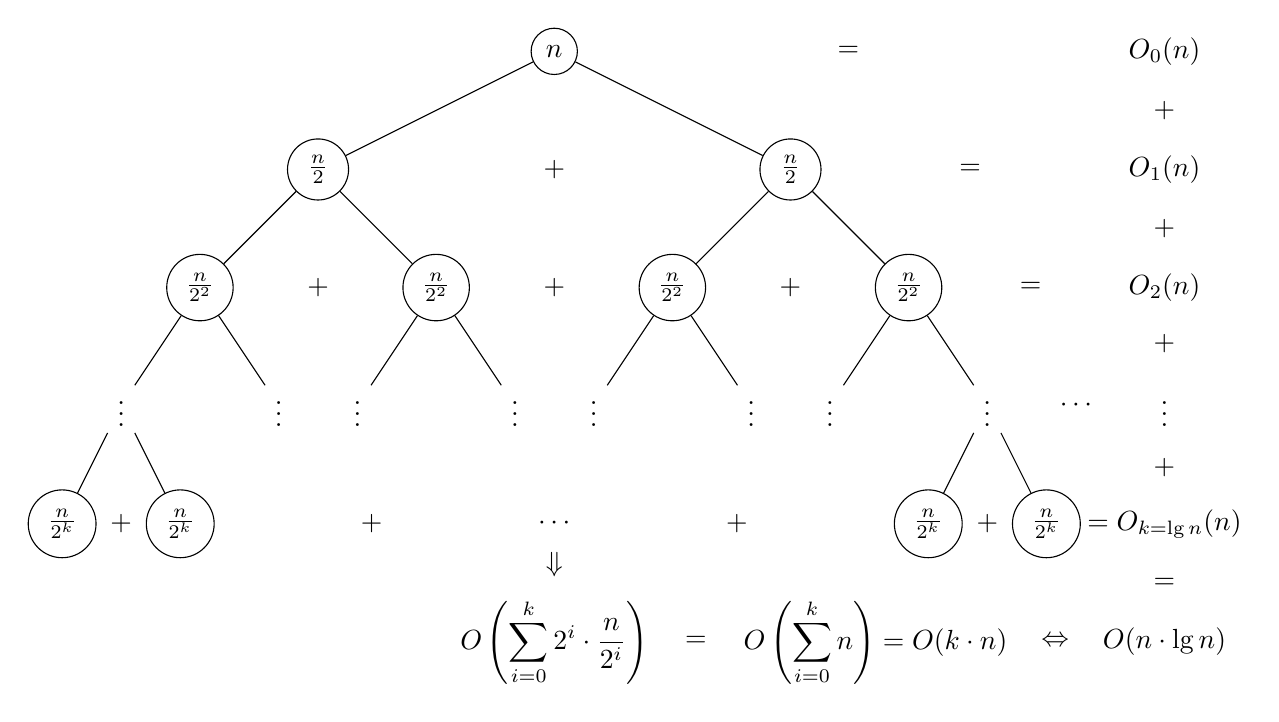
\begin{tikzpicture}[level/.style={sibling distance=60mm/#1}]
			\node [circle,draw] (z){$n$}
			child {node [circle,draw] (a) {$\frac{n}{2}$}
					child {node [circle,draw] (b) {$\frac{n}{2^2}$}
							child {node {$\vdots$}
									child {node [circle,draw] (d) {$\frac{n}{2^k}$}}
									child {node [circle,draw] (e) {$\frac{n}{2^k}$}}
								}
							child {node {$\vdots$}}
						}
					child {node [circle,draw] (g) {$\frac{n}{2^2}$}
							child {node {$\vdots$}}
							child {node {$\vdots$}}
						}
				}
			child {node [circle,draw] (j) {$\frac{n}{2}$}
					child {node [circle,draw] (k) {$\frac{n}{2^2}$}
							child {node {$\vdots$}}
							child {node {$\vdots$}}
						}
					child {node [circle,draw] (l) {$\frac{n}{2^2}$}
							child {node {$\vdots$}}
							child {node (c){$\vdots$}
									child {node [circle,draw] (o) {$\frac{n}{2^k}$}}
									child {node [circle,draw] (p) {$\frac{n}{2^k}$}
											child [grow=right] {node (q) {$ = O_{k = \lg n}(n)$} edge from parent[draw=none]
													child [grow=up] {node (r) {$\vdots$} edge from parent[draw=none]
															child [grow=up] {node (s) {$O_2(n)$} edge from parent[draw=none]
																	child [grow=up] {node (t) {$O_1(n)$} edge from parent[draw=none]
																			child [grow=up] {node (u) {$O_0(n)$} edge from parent[draw=none]}
																		}
																}
														}
													child [grow=down] {node (v) {$O(n \cdot \lg n)$}edge from parent[draw=none]}
												}
										}
								}
						}
				};
			\path (a) -- (j) node [midway] {+};
			\path (b) -- (g) node [midway] {+};
			\path (k) -- (l) node [midway] {+};
			\path (k) -- (g) node [midway] {+};
			\path (d) -- (e) node [midway] {+};
			\path (o) -- (p) node [midway] {+};
			\path (o) -- (e) node (x) [midway] {$\cdots$}
			child [grow=down] {
					node (y) {$O\left(\displaystyle\sum_{i = 0}^k 2^i \cdot \frac{n}{2^i}\right)$}
					edge from parent[draw=none]
				};
			\path (q) -- (r) node [midway] {+};
			\path (s) -- (r) node [midway] {+};
			\path (s) -- (t) node [midway] {+};
			\path (s) -- (l) node [midway] {=};
			\path (t) -- (u) node [midway] {+};
			\path (z) -- (u) node [midway] {=};
			\path (j) -- (t) node [midway] {=};
			\path (y) -- (x) node [midway] {$\Downarrow$};
			\path (v) -- (y)
			node (w) [midway] {$O\left(\displaystyle\sum_{i = 0}^k n\right) = O(k \cdot n)$};
			\path (q) -- (v) node [midway] {=};
			\path (e) -- (x) node [midway] {+};
			\path (o) -- (x) node [midway] {+};
			\path (y) -- (w) node [midway] {$=$};
			\path (v) -- (w) node [midway] {$\Leftrightarrow$};
			\path (r) -- (c) node [midway] {$\cdots$};
		\end{tikzpicture}}
	\caption{Lorem ipsum dolor sit amet}\label{img:index}
\end{figure}
%-------------------------------------------------------------------------------


%-------------------------------------------------------------------------------
% Code
%-------------------------------------------------------------------------------
\begin{lstlisting}[caption={Zbytečný kód},label=list:8-6,captionpos=b,float,abovecaptionskip=-\medskipamount,abovecaptionskip=\medskipamount,language=C]
    #include<stdio.h>
    #include<iostream>
    // A comment
    int main(void)
    {
        printf("Hello World\n");
        return 0;
    }
\end{lstlisting}

%%%%%%%%%%%%%%%%%%%%%%%%%%%%%%%%%
% alternative using package minted for source highlighting
% package minted requires execution with `-shell-escape'
% e.g., `xelatex -shell-escape ctufit-thesis.tex'
% \begin{listing}
% \begin{minted}{C}
%     #include<stdio.h>
%     #include<iostream>
%     // A comment
%     int main(void)
%     {
%         printf("Hello World\n");
%         return 0;
%     }
% \end{minted}
% \caption{Zbytečný kód}\label{list:8-6}
% \end{listing}
% %%%%%%%%%%%%%%%%%%%%%%%%%%%%%%%%%

%-------------------------------------------------------------------------------
% Table
%-------------------------------------------------------------------------------
\begin{table}\centering
	\begin{tabular}{l|l|c|c}
		Typ       & Prostředí          & \LaTeX{}ovská zkratka & \TeX{}ovská zkratka	\tabularnewline \hline
		Text      & \verb|math|        & \verb|\(...\)|        & \verb|$...$|	\tabularnewline \hline
		Displayed & \verb|displaymath| & \verb|\[...\]|        & \verb|$$...$$|	\tabularnewline
	\end{tabular}
	\caption[Příklad tabulky]{Zadávání matematiky}
	\label{tab:matematika}
\end{table}
\begin{landscape} % package pdflscape
	\begin{table}\centering
		% zalamování p{šířka}
		% vertikální centrování pomocí balíčku array
		\begin{tabular}{p{.65\textwidth}|l|c|c}
			\textbf{Typ} & Prostředí          & \LaTeX{}ovská zkratka & \TeX{}ovská zkratka	\tabularnewline \hline\hline
			Text         & \verb|math|        & \verb|\(...\)|        & \verb|$...$|	\tabularnewline \hline
			Displayed    & \verb|displaymath| & \verb|\[...\]|        & \verb|$$...$$|	\tabularnewline
		\end{tabular}
		\caption[Příklad tabulky]{Zadávání matematiky}
		\label{tab:matematika2}
	\end{table}
\end{landscape}

%-------------------------------------------------------------------------------
\paragraph{Nadpis 5. úrovně}

%-------------------------------------------------------------------------------
\begin{definition}[Optional label]

\end{definition}

\begin{example}

\end{example}


\begin{theorem}

\end{theorem}

\begin{proof}

\end{proof}

\paragraph{Level 5 heading}

\begin{corollary}

\end{corollary}

\begin{proposition}

\end{proposition}

\begin{note}

\end{note}

\begin{remark}

\end{remark}

\begin{lemma}

\end{lemma}

\begin{description}
	\item[Chapter 1] I don't know
\end{description}
%-------------------------------------------------------------------------------

\begin{listing} % Package minted
	\begin{verbatim}
Everything in this block is outputed the sam way as it's here
\end{verbatim}
	\caption{}
	\label{}
\end{listing}



\appendix\appendixinit{} % do not remove these two commands

\chapter{Nějaká příloha}


Sem přijde to, co nepatří do hlavní části.
 % include `appendix.tex' from `text/' subdirectory

\backmatter{} % do not remove this command

% print out the BibLaTeX-generated bibliography list
\printbibliography{}

\chapter{Obsah příloh}
% Contents of the attachment

	\dirtree{%
		.1 /.
		.2 readme.txt\DTcomment{stručný popis obsahu média}.
		.2 exe\DTcomment{adresář se spustitelnou formou implementace}.
		.2 src.
		.3 impl\DTcomment{zdrojové kódy implementace}.
		.3 thesis\DTcomment{zdrojová forma práce ve formátu \LaTeX{}}.
		.2 text\DTcomment{text práce}.
		.3 thesis.pdf\DTcomment{text práce ve formátu PDF}.
	}
 % include `medium.tex' from `text/' subdirectory

\end{document}
